\documentclass[reqno]{amsart} \input{common.tex}

% \usepackage{tikz-cd}

\begin{document}

\title{Aarhus Automorphic Forms Conference}

\begin{abstract}
  Partial notes on some of the lectures.  These notes are incomplete, have not been proofread, and should be considered only a crude approximation to what happened in the lectures, filtered through my own misunderstandings and distractions.  Any errors should be assumed to be due to the note-taker.  Corrections welcome!
\end{abstract}


\section{Peter Koymans, \emph{Hilbert 10 via additive combinatorics}}


Let's start with a question of Hilbert from the influential 1900 conference:
\begin{question}
  Does there exist an algorithm with
  \begin{itemize}
  \item INPUT: $f \in \mathbb{Z}[x_1, \dotsc, x_n]$
  \item OUTPUT: ``YES'' if there is a solution $a_1, \dotsc, a_n \in \mathbb{Z}$ to $f(a_1, \dotsc, a_n) = 0$, ``NO'' if not?
  \end{itemize}  
\end{question}
Let's give a brief overview of the history of this question:
\begin{definition}
  A subset $S \subseteq \mathbb{Z}$ is called \emph{Diophantine} if there exists an integer $m > n$ and a polynomial $f \in \mathbb{Z}[x_1, \dotsc, x_n]$ such that
  \begin{equation*}
    S = \left\{(a_1, \dotsc, a_n) \in \mathbb{Z}^n \mid \text{ there exists } a_{n + 1, \dotsc, a_m} \in \mathbb{Z}, \, f(a_1, \dotsc, a_m) = 0 \right\}.
  \end{equation*}
  In other words, take the solution set to a polynomial equation and project it onto some coordinates.
\end{definition}
A bit of history:
\begin{itemize}
\item 1951 (Julia Robinson): A certain hypothesis \textrm{JR} implies that
  \begin{equation*}
    \mathrm{EXP} := \left\{(a, b, c) \in \mathbb{N}^3 : a = b^{c} \right\}
  \end{equation*}
  is Diophantine.  A key ingredient is Pell's equation.
\item 1960 (DPR): The exponential Diophantine sets are exactly the recursively enumerable \textrm{RE} sets, meaning, those sets all of whose elements can eventually be listed (exactly) by an algorithm if we let it run forever.  
\item A corollary of this is that \textrm{JR} implies that Hilbert's 10th problem is undecidable.  For instance, the Halting Problem is \textrm{RE}.
\item 1970 (Matiyasevich): Proved \textrm{JR}.
\end{itemize}
\begin{theorem}[Mazur--Rubin]
  Let $R$ be a finitely-generated ring over $\mathbb{Z}$, with $\lvert R \rvert = \infty$.  Assume that for all number fields $K$, and all elliptic curves $E$ over $K$, that the Tate--Shafarevich group $\operatorname{Sha}(E/K)$ is finite.  Then Hilbert's 10th problem is undecidable over $R$.
\end{theorem}
\begin{theorem}[Koymans–Pagano, 2024]\label{theorem:cq6vrxrm1j}
  Same result, unconditionally.  
\end{theorem}
\begin{theorem}[Koymans–Pagano, 2024]\label{theorem:cq6vrxro7z}
  Let $K$ be a number field.  Then $\mathbb{Z}$ is Diophantine over $\mathcal{O}_K$
\end{theorem}
Let
\begin{theorem}[Koymans–Pagano]\label{theorem:cq6vrxrob0}
  Let $K$ be a number field with $\geq 32$ real embeddings.  Then there exists $E/K$ such that $\operatorname{rank} E(K)  = \operatorname{rank} E(K(i)) > 0$.
\end{theorem}
The proof that Theorem \ref{theorem:cq6vrxrob0} implies Theorem \ref{theorem:cq6vrxrm1j} uses the following:
\begin{lemma}
  Let $K \subseteq L$ be number fields.  Then:
  \begin{enumerate}[(i)]
  \item\label{enumerate:cq6vr0vqg9} If $D_1$, $D_2$ are Diophantine over $\mathcal{O}_K$, then so is $D_1 \cap D_2$.
  \item\label{enumerate:cq6vr0zdtm} If $D \subseteq \mathcal{O}_K$ is Diophantine over $\mathcal{O}_K$, and also $\mathcal{O}_K$ is Diophantine over $\mathcal{O}_L$, then $D$ is Diophantine over $\mathcal{O}_L$.
  \item\label{enumerate:cq6vrx9ccs} If $\mathbb{Z}$ is Diophantine over $\mathcal{O}_L$, then $\mathbb{Z}$ is Diophantine over $\mathcal{O}_K$.
  \item\label{enumerate:cq6vr0ybj9} If $K$ is totally real, then $\mathbb{Z}$ is Diophantine over $\mathcal{O}_K$.
  \item\label{enumerate:cq6vr0twgm} If $E$ satisfies $\operatorname{rank} E(K) = \operatorname{rank} E(L) > 0$, then $\mathcal{O}_K$ is Diophantine over $\mathcal{O}_L$.
  \end{enumerate}
\end{lemma}
Assuming the above:
\begin{proof}[Proof that Theorem \ref{theorem:cq6vrxrob0} implies Theorem \ref{theorem:cq6vrxrm1j}]
  Let $K$ be a number field.  We want to show that $\mathbb{Z}$ is Diophantine over $\mathcal{O}_K$.  Define $M$ to be the Galois closure of $K(i, \sqrt{2}, \dotsc, \sqrt{13})$.  It suffices to show that $\mathbb{Z}$ is Diophantine over $\mathcal{O}_M$, by \eqref{enumerate:cq6vrx9ccs}.  Taking the decomposition group $D \subseteq \Gal(M / \mathbb{Q})$ at an infinite place, we must have $1 \notin M^D =: L$.  Thus $M = L(i)$.  Hence by Theorem \ref{theorem:cq6vrxrob0} and \eqref{enumerate:cq6vr0twgm}, we know that $\mathcal{O}_{M^D}$ is Diophantine over $\mathcal{O}_M$.  Hence by \eqref{enumerate:cq6vr0vqg9}, we see that
  \begin{equation*}
    \bigcap_{
      \substack{
        D \subseteq \Gal(M / \mathbb{Q})  \\
        D \text{ decomp. at } \infty
      }
    }
    \mathcal{O}_D.
  \end{equation*}
  is Diophantine over $\mathcal{O}_M$.  We may write the above as $\mathcal{O}_F$, with
  \begin{equation*}
    F := \bigcap_{
      \substack{
        D \subseteq \Gal(M / \mathbb{Q})  \\
        D \text{ decomp. at } \infty
      }        
    }
    M^D.
  \end{equation*}
  But $F$ is totally real, so $\mathbb{Z}$ is Diophantine over $\mathcal{O}_F$ by \eqref{enumerate:cq6vr0ybj9}, hence $Z$ is Diophantine over $\mathcal{O}_M$ by \eqref{enumerate:cq6vr0zdtm}.
\end{proof}

Let's now give the proof of Theorem \ref{theorem:cq6vrxrob0}.

\textbf{We first discuss $2$\emph{-Selmer groups}}.  Take the Galois cohomology of $G_K := \Gal(\bar{K} / K)$.  Look at
\begin{equation*}
  0 \rightarrow E[2] \rightarrow E \xrightarrow{\bullet 2} E \rightarrow 0.
\end{equation*}
This gives
\begin{equation*}
  0 \rightarrow E(K)[2] \rightarrow E(K) \xrightarrow{\bullet 2} E(K) \xrightarrow{\delta} H^1(G_{K}, E[2]),
\end{equation*}
so
\begin{equation*}
  0 \rightarrow
  \frac{E(K)}{2 E(K)}
  \xrightarrow{\delta} H^1(G_K, E[2]).
\end{equation*}
The first term is an $\mathbb{F}_2$-vector space of dimension
\begin{equation*}
  \operatorname{rank} E(K) + \dim_{\mathbb{F}_2} E(K)[2].
\end{equation*}
We can also do the same diagram for each place $v$ of $K$.  You can check that this whole thing gives a commutative diagram
\begin{equation*}
  \begin{CD}
    \small
    0 @>>> E(K)[2] @>>> E(K) @>{\bullet 2}>> E(K) @>{\delta}>> H^1(G_K, E[2]) \\
    @. @VVV @VVV @VV \res_vV @VV\res_vV \\
    0 @>>> E(K_v)[2] @>>> E(K_v) @>{\bullet 2}>> E(K_v) @>{\delta_v}>> H^1(G_{K_v}, E[2])
  \end{CD}
\end{equation*}<++>
\begin{equation*}
  0 \rightarrow E(K)[2] \rightarrow E(K) \xrightarrow{\bullet 2} E(K) \xrightarrow{\delta} H^1(G_K, E[2])
  \xrightarrow{\res_v}
  H^1(G_{K_v}, E[2])
\end{equation*}
and
\begin{equation*}
  0 \rightarrow  E(K_v)[2]
  \rightarrow E(K_v) \xrightarrow{\bullet 2}
  E(K_v)
  \xrightarrow{\delta_v} H^1(G_{K_v}, E[2]).
\end{equation*}
Hence $\Sel^2(E / K) := \ker(H^1(G_K, E[2]) \xrightarrow{\prod \res_v} H^1(G_{K_v}, E[2]) / \image(\delta_v))$.
\begin{enumerate}
\item If $\image(\delta) \subseteq \Sel^2(E / K)$, then $\rank E(K) + \dim_{\mathbb{F}_2} E(K)[2] \leq \dim_{\mathbb{F}_2} \Sel^2(E / K)$.
\item $\Sel^2(E / K)$ is computable and finite-dimensional.
\end{enumerate}

\textbf{Let's now discuss \emph{forcing positive rank}}.  Take $\tilde{E}$ with $\tilde{E}(K)[2] \cong \mathbb{F}_2^2$, i.e., $y^2 =(x - a_1)(x - a_2)(x - a_3)$ with $a_1, a_2, a_3 \in K$ distinct.  Twisting by $t :=(n - a_1)(n - a_2)(n - a_3)$ gives a new elliptic curvge $t y^2 =(x - a_1)(x - a_2)(x - a_3)$ with rational point $(x, y) =(0, 1)$.  Twisting by $t :=(n - a_1 d)(n - a_2 d)(n - a_3 d)$ gives a new curve with rational point $(x, y) =(\tfrac{n}{d}, \tfrac{1}{d^2})$.

Since $i \notin K$, we have $\operatorname{rank} \tilde{E}^t(K(i)) = \rank \tilde{E}^t(K)$ suffices to find $t = d(n - a_1 d)(n - a_2 d)(n - a_3 d)$ with $\rank \tilde{E}^{- t}(K) = 0$.  It suffices to show that $\dim_{\mathbb{F}_2} \Sel^2(E/K) = 2$, because this implies that $\rank \tilde{E}^{- t}(K)[2] + 2 \leq 2$, whence $\rank \tilde{E}^{- t}(K)[2] = 0$.

So we need to control $2$-Selmer groups.  What's the punchline?  (We've talked about Hilbert 10, but not yet additive combinatorics.)  \textbf{Fact}: we can compute $\Sel^2(E / K)$ from Legendre symbols of primes dividing $t$.

\section{Morten Risager, \emph{The error term in the hyperbolic circle problem}}

Let $\Gamma \leq \mathrm{SL}_2(\mathbb{R})$ be a discrete, cofinite subgroup that contains $- 1$.  A good example is $\mathrm{SL}_2(\mathbb{Z})$.

Let $z, z ' \in \mathbb{H}$.  We want to count how many $\Gamma$-translates of $z$ lie in a hyperbolic circle based at $z'$, with radius $R \rightarrow \infty$:
\begin{equation*}
  N(z, z', X)
  :=
  \#
  \left\{
    \gamma \in \Gamma \mid
    4 u(\gamma z, z ') + 2 \leq X
  \right\}.
\end{equation*}
Here $u(z, z') = \frac{\lvert z - z ' \rvert^2}{4 \Im(z) \Im(z')}$.
We note that  $4 u(\gamma z, z ') = 2 \cosh(d_H(\gamma z, z '))$, so one can formulate the counting problem in a few ways.

Selberg (1970's) showed that
\begin{equation*}
  N(z, z', X)
  =
  \frac{2 \pi}{\vol(\Gamma \backslash \mathbb{H})}
  X
  +
  (\text{contribution from small eigenvalues})
  + \O(X^{2/3}).
\end{equation*}
(Selberg never published this result, but he gave talks about it, and we have notes from these talks available at the IAS.)

\begin{question}
  Can $\O(X^{2/3})$ be improved?  (Note that $\tfrac{2}{3} = \tfrac{1}{2} + \tfrac{1}{6}$.)
\end{question}

We have the $\Omega$-result of Phillips--Rudnick ('94): $N(z, z', X) - M(X) = \Omega(X^{\frac{1}{2} - \delta})$, for each $\delta > 0$.

What do we do when we don't know how to bound something?  We try to do something easier: take an average of some sort.  Look at the second radial moment.

Chamizo ('96):
\begin{equation*}
  \left( \frac{1}{X} \int_X^{2 X} \left( N(z, z', X) - M(X) \right)^2 \, d x  \right)^{1/2}
  = \O\bigl(
  X^{1/2} \log X\bigr).
\end{equation*}
Cherubini (2016):
\begin{equation}\label{eq:cq6vse71xz}
  \O(X^{1/2} \log^{1/2} X).
\end{equation}

\begin{conjecture}
  $N(z, z', X) - M(X) = \O(X^{\frac{1}{2} + \eps})$.
\end{conjecture}

\textbf{Local averages}.  Biro (2018): take $f$ of compact support, and $z = z '$.  Then
\begin{equation*}
  \int_{\Gamma \backslash \mathbb{H}}
  f(z) \left( N(z, z, X) - M(X) \right)
  \, d \mu(z)
  = \O\bigl(X^{\frac{1}{2} + \frac{1}{8}}\bigr).
\end{equation*}

From now on, restrict to $\Gamma = \mathrm{SL}_2(\mathbb{Z})$.  In that case, the main term is simply $6 X$.  One can improve Phillips--Rudnick to $\Omega\bigl(X^{\frac{1}{2}}(\log X)^{\frac{1}{4} - \delta}\bigr)$ , and Cherubini to $\O(X^{\frac{1}{2} + \frac{1}{12} + \eps})$.

We want now to restrict to an even more arithmetic situations, where $z = z_d$ and $z ' = z_{d '}$ are both Heegner points.  We want $d$ and $d'$ to be different fundamental squarefree discriminants, with $0 > d = b^2 - 4 a c \equiv 1 \pmod{4}$ and
\begin{equation*}
  z_d = \frac{- b + \sqrt{\lvert d \rvert}}{2 a}.
\end{equation*}
\begin{theorem}
  Second spacial moment: with $\Gamma = \mathrm{SL}_2(\mathbb{Z})$,
  \begin{equation*}
    \Bigl( \int_{\Omega} \bigl( N(z, z, X) - M(X) \bigr)^2 \, d \mu(z) \Bigr)^{1/2} = \O(X^{\frac{1}{2} + \frac{1}{7}}).
  \end{equation*}  
\end{theorem}

Let's return to the theorem:
\begin{theorem}[Chatzakos, Cherubini, Lester, Risager, 2025]
  Let $\Gamma = \mathrm{SL}_2(\mathbb{Z})$, and $d$, $d'$ are as above.  Then we manage to prove
  \begin{equation*}
    N(z_d, z_{d'}, X) = b X + \O(\frac{X^{2/3}}{(\log X)^{1/6}}).
  \end{equation*}
\end{theorem}
We can furthermore  improve \eqref{eq:cq6vse71xz} to $\O\bigl(X^{1/2} \log^{3/8} X\bigr)$
\begin{itemize}
\item $p_0(x, y) := a_0 x^2 + b_0 x y + c_0 y^2$, $d_0 = b_0 4 a_0 c_0$
\item $p(x, y) = a x^2 + b x y + c y^2$, $d = b^2 - 4 a c$
\item $\mathrm{codiscr}(p, p) = 2(a c_0 - c a_0) - b b_0$.
\end{itemize}
\begin{corollary}
  Fix $d$, $d_0$ (not equal to $-3$ (different squarefree fundmental discriminants).
  \begin{equation*}
    \eta_d = \left\{ p \mid a > 0, \, \text{discr}(p) = d,
      \,
      0 <(\sigma - \operatorname{discr(p, p_0)})\right\}
    = \frac{6 h(d)}{ \sqrt{d d_0}}
    + \O(\frac{X^{2/3}}{(\log q k^{1/2})}).
  \end{equation*}
\end{corollary}
To understand $N(z, z', X)$, it is useful to understand bounds on
\begin{equation*}
  S(x) := \sum_{T \leq t_j \leq 2 T}
  \sum_{T \leq t_j \leq 2 T}
  X^{t_j}
  \varphi_j(z) \overline{\varphi_j(z ')}
  \ll T^2.
\end{equation*}
Here $\lambda_j = \tfrac{1}{4} + j^2$ is an eigenvalue of $\Delta_P$ with eigenfunction $q_j(z)$.

We prove:
\begin{equation*}
  \lvert S(X, T) \rvert
  \leq \sum_{T \leq t_j \leq 2 T}
  \left\lvert \varphi_{j}(z_d) \varphi_j(z_{d '}) \right\rvert
  \ll \frac{T^2}{(\log T)^{1/4}}.
\end{equation*}

Using Waldspurger:
\begin{equation*}
  \lvert \varphi_j(z) \rvert \ll_d  \sum_{\xi \in \widehat{\mathrm{Cl}(\mathbb{Q}(\sqrt{d}))}}
  \frac{L(\varphi_j \times f_\xi, \frac{1}{2})^{\frac{1}{2}}}{L(1, \sym^2 \varphi_j)}.
\end{equation*}
Here $f_s$ is the theta series related to the class group character $\xi$.

\begin{theorem}
  Let $d$ and $d'$ be different, $\xi \in \widehat{\mathrm{Cl}(\mathbb{Q}(\sqrt{d}))}$ and $\xi' \in \widehat{\mathrm{Cl}(\mathbb{Q}(\sqrt{d'}))}$.  Then
  \begin{equation*}
    \sum_{T \leq t_j \leq 2 T}
    \frac{L(\varphi_j \times f_\xi, \frac{1}{2})^{1/2} L(\varphi_j, f_{\xi '})^{1/2}}{L(\sym^2 \varphi_j, 1)}
    = \O\left( \frac{T^2}{(\log T)^{1/4}}\right)
  \end{equation*}
\end{theorem}
In order to prove this, we needed
\begin{equation*}
  \sum_{t_j} h(t_j) \frac{L(\tfrac{1}{2}, \varphi_j \times f_{\xi})}{L(\sym^2 \varphi, 1)}
  \lambda_j(\ell) = C_h
  \frac{\lambda_{f_{\xi}}(\ell)}{\sqrt{\ell}} T^2 + \O(T^{1 + \eps}).
\end{equation*}
Here $h$ localizes at $[T, 2 T]$.

\section{Alan Zhao, \emph{A different perspective on Whittaker functions for} $\mathrm{GL}_n$}

\subsection{Notation}

Let $\lambda$ denote a partition, say $(4 3 1)$, with accompanying Young diagram.  We'll also use
\begin{equation*}
  (a;q) =(1 - a)(1 - a q) \dotsb(1 - a q^{n - 1}).
\end{equation*}
We'll also fix $q < 1$.

To introduce the $q$-deformation Whittaker functions, we'll start by defining:
\subsection{MacDonald polynomials}
These will lie in $\mathbb{Q}(q, t)[x_1, \dotsc, x_n]$.  They'll depend upon a partition, whose length is the number of variables.  For each $\lambda$, there exists $P_\lambda$ such that $\langle P_\lambda, P_\mu \rangle = 0$ for $\lambda \neq \mu$.  We get $P_\lambda(x, q, t)$.  Specializations:
\begin{itemize}
\item $q = 0 \rightsquigarrow$ Hall--Littlewood.
\item $t = 0 \rightsquigarrow$ $q$-Whittaker.
\item Applying both, we obtain Schur polynomials.
\end{itemize}

\begin{example}
  The $q$-Whittaker polynomial associated to $\lambda =(2 1)$ is
  \begin{equation*}
    (x_1^3 + x_2^3) +(1 + q + q t)(x_1^2 x_2 + x_1 x_2^2).
  \end{equation*}
  If you just take $q = 1$ naively, you get (...).)
\end{example}

$q$-Whittaker $\Psi_{x_1, \dotsc, x_n}(\underline{\lambda}_n)$, where $\underline{\lambda}_n$ is a Gelfand--Tsetlin pattern $\lambda_{n, 1} \geq \lambda_{n, 2} \geq \dotsb \lambda_{n, n}$ with interlaced rows below that.  This comes out to
\begin{equation*}
  \Psi_{x_1, \dotsc, x_n}(\underline{\lambda}_n) = \sum_{\text{patterns}} \prod x_i^{\sum \lambda_{???} - \sum_{?}\lambda_{\dotsb}}
  \times(\text{quotient of }(q, q)_n).
\end{equation*}


\section{Valentin Blomer, \emph{Hecke fields - Galois theory meets shifted convolution problems}}

Let $f(z) = \sum_n a_n e(n z)$ be a cusp form, $\mathbb{Q}(f) := \mathbb{Q}(\left\{ a_n \mid n \in \mathbb{N}  \right\})$.

Let $\chi$ be a Dirichlet character, $\mathbb{Q}(\chi) := \mathbb{Q}(\left\{ \chi(n) \mid n \in \mathbb{N} \right\})$.

Shimura (1977): there exists $\Omega_{f, \pm} \in \mathbb{C}^\times$ such that
\begin{equation*}
  L^{\mathrm{alg}}(\tfrac{1}{2}, f \times \chi)
  :=
  \frac{G(\bar{\chi}) L(\tfrac{1}{2}, f \times \chi)}{\Omega_{f, \sgn(\chi)}}
  \in \mathbb{Q}(f, \chi).
\end{equation*}
Here we think of $f$ as being fixed and $\chi$ as varying.  Moreover, we have the following \emph{reciprocity}: for a Galois automorphism $\sigma$,
\begin{equation*}
  \sigma L^{\mathrm{alg}}(\tfrac{1}{2}, f \times \chi)
  := L(\tfrac{1}{2}, f^\sigma \times \chi^\sigma).
\end{equation*}

We recall that
\begin{equation*}
  \mathbb{Z}_p^\times = \mu_{p - 1} \times(1 + p \mathbb{Z}_p)
  \cong \widehat{\mathbb{Z}^\times_p}.
\end{equation*}
If we take a character $\chi$ of prime power conductor $p^{h}$, then $p^{h - 1}$ divides the order of $\chi$.  We're interested in the set of characters $\chi$ such that the conductor is $p^{h}$ and the order is $p^{h - 1}$:
\begin{equation*}
  \Xi_{p, h} := \left\{ \chi : \mathrm{conductor} = p^{h}, \mathrm{order} = p^{h - 1} \right\}.
\end{equation*}
In the terminology of Ravi's talk yesterday, these are ``wild characters''.  We'll see later that this is a Galois orbit.  The values of such a character $\chi$ are $p^{h - 1}$th roots of unity, and most of these values are primitive.  In particular,
\begin{equation*}
  \operatorname{image}(\chi) = \mu_{p^{h - 1}}.
\end{equation*}
More precisely, $\chi(x)$ is a primitive $p^{h - 1}$ root of unity if and only if $x = x_0 + x_1 p + x_2 p^2 + \dotsb$, where $p \nmid x_0 x_1$.

After this interlude on characters, we come to the thing we really want to discuss.  The number $L^{\mathrm{alg}}(\tfrac{1}{2}, f \times \chi)$ lies in the field $\mathbb{Q}(f, \chi)$, and you might ask, is it a generator of the field?  When is this the case?

The work of Luo--Ramakrishnan (1977) and later work of Sun (2019) established the following.  Fix a prime $p$ and a cusp form $f$.  We make the assumption that $f$ has no inner twist, meaning that $f$ is not equal to $f \otimes \chi_D$ for a real character $\chi_D$.  (If the level is squarefree, then this can never happen.)  Then they proved that $\mathbb{Q}(f, \chi) = \mathbb{Q}(L^{\mathrm{alg}}(\tfrac{1}{2}, f \times \chi), \mu_p)$ holds for all $\chi \in \Xi_{p, h}$ provided that $h \geq h_0$.  That's quite remarkable - a central character is able to generate fields when you run through character.

We want to do the same with more complicated expressions involving this central value (see \cite{2025arXiv2503.15040}):
\begin{theorem}[Blomer--Burungale--Michel--Min]
  Under the same assumptions, $\mathbb{Q}(f, \chi) = \mathbb{Q}(\left\lvert L(\tfrac{1}{2}, f \times \chi) \right\rvert^2, \mu_p)$ for all $\chi \in \Xi_{p, h}$ with $h \geq h_0$.
\end{theorem}
We note that the containment ``$\supseteq$'' is obvious; the hard part is to show ``$\subseteq$''.

As announced in the abstract, there is an analytic part and a Galois-theoretic part.

\subsection{Galois theory}
We have $\mathbb{Q}(\chi) \subseteq \mathbb{Q}(\mu_p, \ast)$ and $\mathbb{Q}(f) \subseteq \mathbb{Q}(\chi, \ast)$.  The real reason we picked this topic is that we can now draw complicated field diagrams.

The top field is $\mathbb{Q}(f, \chi)$, which contains $\mathbb{Q}(\chi, \ast)$.  This contains $\mathbb{Q}(\chi)$ (branching down and to the left) and also $\mathbb{Q}(\mu_p , \ast)$ (branching down and to the right), which both contain the common subfield $\mathbb{Q}(\chi) \cap \mathbb{Q}(\mu_p, \ast)$, which in turn contains $\mathbb{Q} $.  There is a further extension, with dotted lines: $\mathbb{Q}(f, \chi)$ contains $\mathbb{Q}(f)$ which contains $\mathbb{Q}$.  Furthermore, $\mathbb{Q}(f)$ is contained in its Galois extension $E$, which is contained in (branching up and to the right) $E(\chi)$, which contains (down and to the right) $\mathbb{Q}(f, \ast)$, and then there's the common subfield $E \cap \mathbb{Q}(\chi, \ast)$ of $E$ and $\mathbb{Q}(f, \ast)$:

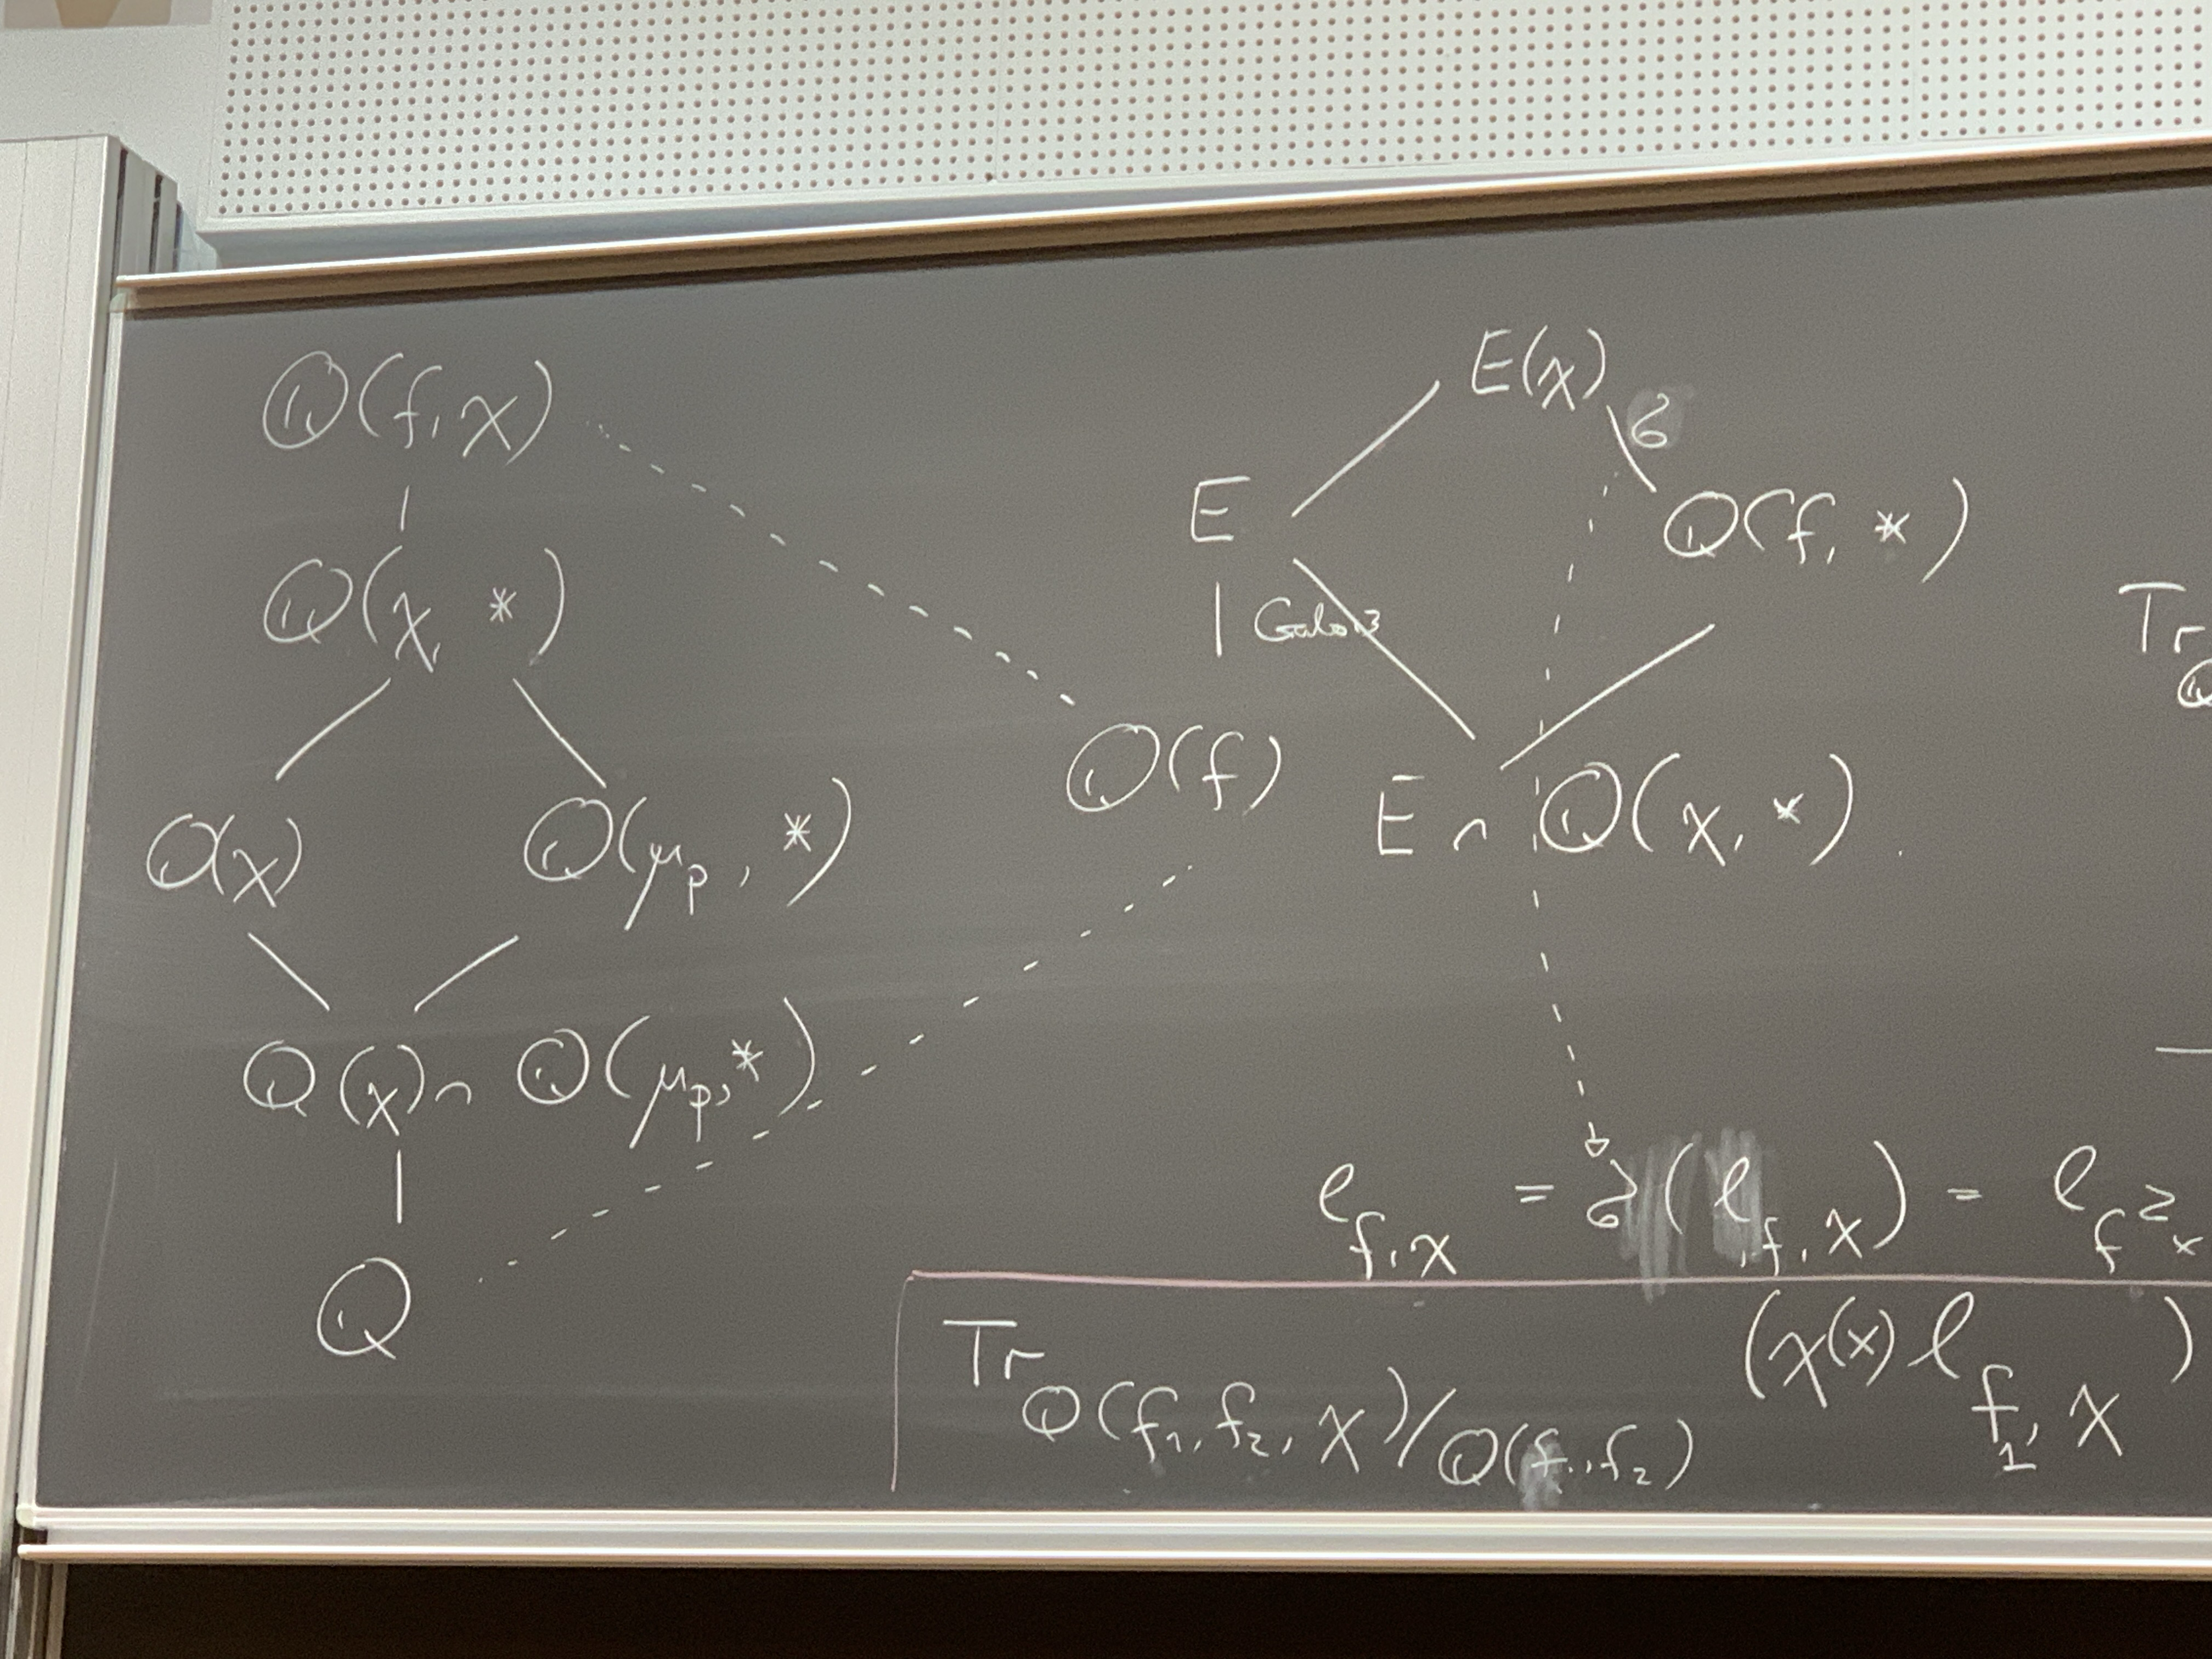
\includegraphics[width=0.5\textwidth]{images/img_20250813_094513}

We set $\ell_{f, \chi} := \lvert L^{\mathrm{alg}}(\tfrac{1}{2}, f \times \chi) \rvert^2$.  By some diagram chasing, we have
\begin{equation*}
  0 \neq \trace_{\mathbb{Q}(f, \chi) / \mathbb{Q}}(\chi(x) \ell_{f, \chi})
  = \trace_{\mathbb{Q}(\mu_p, \ast) / \mathbb{Q}} \left( \ell_{f, \chi} \trace_{\mathbb{Q}(f, \chi) / \mathbb{Q}(\mu_p, \ast)} \chi(x) \right).
\end{equation*}
We deduce that, unless the extension is trivial, we obtain
\begin{equation*}
  \deg \trace_{\mathbb{Q}(\chi, \ast) / \mathbb{Q}(\mu_p, \ast)} \chi(x) = 0.
\end{equation*}
Let $\sigma$ be a Galois automorphism of $E(\chi) / \mathbb{Q}(f, \ast)$.  Then
\begin{equation*}
  \ell_{f, \chi} = \sigma(\ell_{f, \chi}) = \ell_{f^2 \times \chi},
\end{equation*}
which implies that $f = f^\sigma$, so that the extension is trivial.  We then consider
\begin{equation*}
  \trace_{\mathbb{Q}(f_1, f_2, \chi) / \mathbb{Q}(f_1, f_2)}(\chi(x) \ell_{f_1, \chi}).
\end{equation*}
The upshot is that we need to evaluate
\begin{equation}\label{eq:cq6v8d8hcu}
  \sum_{\sigma \in \Gal(F(\chi)) / F_0}
  L(\tfrac{1}{2}, f \times \chi^\sigma) \overline{F(\tfrac{1}{2}, g \times \chi^\sigma)} \chi^\sigma(x).
\end{equation}
We're not summing over all characters, but only over a Galois orbit, so there is only some orthogonality:
\begin{equation*}
  \mathbb{E}_{\sigma} \chi^\sigma(n) := \delta_{n^{p - 1} \equiv 1 \pmod{p^{h}}}.
\end{equation*}

\subsection{Shifted convolution sums}

The standard way to evaluate such a sum of $L$-values is via the approximate functional equation.  This leads morally to something like
\begin{equation}\label{eq:cq6v8a8450}
  \sum_{ \substack{
      m n \leq q^2  \\
      \alpha m \equiv x n \pmod{q}
    } } \lambda_f(m) \lambda_f(n),
\end{equation}
where $x$ is fixed, $q = p^{h}$ and $\alpha^{p - 1} \equiv 1 \pmod{q}$.  The subtlety here is that $\alpha$ is not fixed -- there are only so many such roots of unity, but they're spread out all over the place.  Most results concerning the shifted convolution problem apply when the coefficients playing the role of $\alpha$ and $x$ in \eqref{eq:cq6v8a8450} are essentially fixed.

Let's start with the case $\alpha = 1$.  Take $n \asymp N$, $m \asymp M$.
\begin{enumerate}[(i)]
\item\label{enumerate:cq6v8blrg4} If $N \leq q^{3/2 - \eps}$, then one can apply spectral methods: $\delta$-symbol, Voronoi summation, large sieve.  Indeed, this works as long as the longer variable is no more than three times as long as the shorter variable.
\item\label{enumerate:cq6v8blt69} If $N \geq q^{3/2 + \eps}$, then we apply Voronoi in $n$, which leads to $\frac{N}{q^2} \sum_{m \asymp M} \sum_{n \asymp q^2 / N} \lambda(m) \lambda(n) S(m, n, q)$, which we can treat using the Weil bound for Kloosterman sums.
\item\label{enumerate:cq6v8blu1b} There remains the intermediary range.  One can hope to treat this by upgrading the treatment of the $N \geq q^{3/2 + \eps}$ range, using that $q = p^{h}$ is factorable, via Weyl differencing.
\end{enumerate}
For $\alpha \neq 1$ large, the treatment of case \eqref{enumerate:cq6v8blrg4} breaks down completely.  Without a better idea how to proceed, we take absolute values:
\begin{equation*}
  \sum_{(m, n) \in \Lambda}\lvert \lambda_f(n) \lambda_f(m) \rvert,
  \quad
  \Lambda := \left\{ \alpha m \equiv x n \pmod{q} \right\}.
\end{equation*}
We observe that $\Delta$ is a ``roundish'' lattice, and we're summing nonnegative multiplicative functions over it.  Sieve theory tells us that we understand this, and the answer doesn't depend upon the shape of the lattice.  Recall that (by approximations to Sato--Tate) the magnitudes $\lvert \lambda_f(n) \rvert$ are a bit smaller than $1$ on average.  This saves $(\log q)^{- \delta}$ for some $\delta \approx 0.1$.

This suffices for an asymptotic evaluation of the moment \eqref{eq:cq6v8d8hcu}.  (We were worried that we already had to do a dyadic subdivision, so saving the fractional log would be swamped by the logarithmically many scales, but it turns out that the main term is of size $q \log q$, so it really suffices.)

So, what is the upshot, or the moral to be learned?  There's somehow an interesting passage from generation of Hecke fields to moments -- by a bit of Galois theory, we can relate such a generation question to moments of $L$-functions, at which point we can apply analytic theory.  It results in situations where we're summing over a Galois orbit, which changes the shifted convolution structure drastically.

\section{Zvi Shem-Tov, \emph{Equidistribution of lifts on hyperbolic 4-manifolds}}

(Joint with de Faveri)

Take $M = \Gamma \backslash \mathbb{H}^n$, where $\Gamma = \mathbb{G}(\mathbb{Z})$ and $G = \mathbb{G}(\mathbb{R}) = \SO(1, n)$.

Take a sequence $\phi_j$ of joint eigenfunctions of the hyperbolic Laplacian $\Delta$ and the family of Hecke operators $\mathcal{H}$.  So that this sequence is nontrivial, we require that $\lvert \lambda_j \rvert \rightarrow \infty$.  We also normalize so that $\lVert \phi_j \rVert_2 = 1$.  We define the probability measures
\begin{equation*}
  \mu_j = \lvert \phi_j \rvert^2 \, d \vol.
\end{equation*}
\begin{question}
  What are the weak-$\ast$ limits of such $\mu_j$?
\end{question}
\begin{conjecture}[Rudnick--Sarnak, ``QUE'', 1995]
  The only such limit is the uniform measure $\mu = d \vol$.
\end{conjecture}
What is known so far?  (We focus on this specific setup, ignoring many others.)
\begin{itemize}
\item When $n = 2$, Lindenstrauss (2005) proved for congruence surfaces that $\mu = c \vol$ for some scalar $c$.  When the surface is compact, we must have $c = 1$.  Soundarajan showed in general (e.g., for for $\mathrm{SL}_2(\mathbb{Z})$) that $c = 1$ (``non-escape of mass'').
\item When $n = 3$, Shem-Tov--Silberman (2023) showed the analogous result for $\Gamma \backslash \mathbb{H}^3$, or more generally, $\Gamma \backslash (\mathbb{H}^2)^r \times(\mathbb{H}^3)^s$.  Non-escape of mass was shown in the master's thesis of Zaman.
\item When $n = 4$, we don't quite have QUE, but we do have some partial results.  Shem-Tov--Silberman showed roughly that any such $\mu$ is a countable combination of measures, each of which is either the uniform measure $d \vol$ or the uniform measure on totally geodesic submanifolds of dimension $3$.  In this case, we also know non-escape of mass (de Faveri--Shem-Tov).
\end{itemize}

In the following work in progress, we can prove QUE in dimension $4$ for a concrete, nontrivial example of such a sequence.
\begin{theorem}[de Faveri--Shem-Tov]
  QUE holds for Pitale lifts.  In fact, all we need to know is that the Hecke eigenvalues are large.  The result applies, for instance, to $\Gamma = \operatorname{SU}_2(\mathbb{Z})$.
\end{theorem}

\textbf{Step 1} is the \emph{microlocal lift}.  Namely, we can lift the measure $\mu$ to a measure $\tilde{\mu}$ on the phase space $\Gamma \backslash G$ in a way such that this lift satisfies two conditions:
\begin{itemize}
\item $\tilde{\mu}$ is $A$-invariant.
\item $\tilde{\mu}$ is a limit of Hecke eigenfunctions.
\end{itemize}
We use a very general construction of Silberman--Venkatesh (although such constructions have a long history).  That's the first step -- once we have this microlocal lift, we can forget the original quotients and just speak of measures on these homogeneous spaces.

\textbf{Step 2} is \emph{ergodic theory} or \emph{measure-rigidity}.  Basically, what we do is to try to classify these $A$-invariant measures, using entropy/recurrence conditions and results of Einsiedler--Lindenstrauss.  What we get out is that $\tilde{\mu}$ is a convex combination of homogeneous measures (i.e., a measure on the orbit of a reasonable reasonable).  What we need to show is then that, for $\pi : G \rightarrow \Gamma \backslash G$ the natural projection, we have $\tilde{\mu}(\pi(L)) = 0$ for certain submanifolds $L \subset G$.  The most general result we know how to prove in this context is the following
\begin{theorem}[Shem-Tov--Silberman]
  Assume that for any subspace $U \subset L$ with irreducible Zariski closure $\bar{U}^Z$, we have that
  \begin{equation*}
    S := \left\{ s \in \mathbb{G}(\bar{\mathbb{Q}} \cap \mathbb{R})
      :
      s \bar{U}^Z = \bar{U}^Z
    \right\}
  \end{equation*}
  is $\tfrac{1}{2}$-weakly small (to be defined below).  Then $\tilde{\mu}(\pi(L)) = 0$.
\end{theorem}
\textbf{Weak smallness} (defined by Marshall in the context of the sup norm problem).  Let $H < G$.  Fix maximal split tori $T_H < T_G$.  For $\eta \in X_\ast(T_G)$, define
\begin{equation*}
  \lVert \eta \rVert_G^\ast := \max_{w \in W_G}
  \left\langle \rho_G, w \eta \right\rangle.
\end{equation*}
Here
\begin{equation*}
  \rho_G := \frac{1}{2} \sum_{\alpha > 0} \dim(\mathfrak{g}_\alpha) \alpha.
\end{equation*}
We similarly define $\lVert \eta \rVert_H^\ast$ for $\eta \in X_\ast(T_H)$.  Using these norms, we define two notions of smallness (where one should think $\alpha = \tfrac{1}{2}$):
\begin{itemize}
\item $H$ is $\alpha$\emph{-tempered} if for all $\eta \in X_\ast(T_H)$, we have that $\lVert \eta \rVert_H^\ast \leq \alpha \lVert \eta \rVert_G^\ast$.
\item $H$ is $\alpha$\emph{-weakly small} if, in addition, either $\dim T_H < \dim T_G$ or $\max_{w \in W_G} \lVert w \eta \rVert_H^\ast < \alpha \lVert \eta \rVert_G^\ast$.
\end{itemize}
To give some geometric intuition, take $\eta \in X_\ast(T_G)$ and $p$ prime.  We can then form the corresponding Hecke operator $\tau = \tau(\eta, p)$.  What's important about this norm is that $\lvert \pi(H) \cap \supp(\tau) \rvert \ll \sum_{ \substack{
    w \in W  \\
    w \eta \in X_\ast(T_H)    
  } } p^{2 \lVert w \eta \rVert_H^\ast}$.

Back to non-concentration.  What we really proved is that $\mu(\pi(L)) = 0$ if the following condition is satisfied: each of the stabilizers $S$ that we saw before is contained in

for all $\eps > 0$ there exists a finite set $J_\eps \in \mathcal{H}$ such that for all $\phi$, we can find $\tau \in J_\eps$ so that
\begin{equation*}
  \frac{\lVert \tau \rVert_{L^1(H)}}{\lambda_\phi} < \eps.
\end{equation*}

Idea (Marshall): take $\tau = \left( \sum_{p \sim P} \tau_p \right)^2$ such that each $\tau_p$ satisfies $\tfrac{1}{2}$-weak smallness.  That way, you hope to make the intersection small.  But this is not a basic Hecke operator -- you can expand it as $\tau = \sum \tau_p^2 + \sum_{p \neq q} \tau_p \tau_q$.  We may assume by some other reasons that $\lambda_p \sim(\supp \tau_p)^{1/2}$.  For the off-diagonal, we use weak smallness.  For the diagonal terms, use temperedness.  The problem is that in our case (dimension $4$), there are some very non-small groups that appear: $H \approx \SO(1, 3) \subset \SO(1, 4)$, which is far from being $\tfrac{1}{2}$-tempered; it is $\tfrac{2}{3}$-tempered?  But $\lambda_p \geq(\supp \tau_p)^{1/2}$.  The reason we find our theorem interesting is that we were nevertheless able to construct new Hecke operators such that the argument still works.  This shows that the $\tfrac{1}{2}$-weakly small condition (used in a lot of other works) is \emph{not} tight.  This gives us hope for at least the following two things:
\begin{itemize}
\item We constructed our Hecke operators using spectral methods, involving the Satake isomorphism.  We hoped that maybe a more conceptual, geometric understanding of the Hecke operators and the geometry of the building will improve this construction.  So, maybe there exist better operators that can be used to prove something for general sequences.
\item Nontrivial upper bounds for $\lVert . \rVert_\infty$ in this case, for $\Gamma \backslash \mathbb{H}^4$.
\end{itemize}
Both of these

\section{Matthew Young, \emph{Shifted convolution problem for Siegel modular forms}}

(joint work with Wing Hong (Joseph) Leung; extremely recent, decided to speak on it just a week ago)

Let $\mathbb{H}_2$ denote the Siegel upper half-space, and $G = \mathrm{Sp}_4(\mathbb{R}) := \left\{ g \in \mathrm{GL}_4(\mathbb{R}) \mid g J g^t = J \right\}$ the symplectic group, where $J = \left(
  \begin{smallmatrix}
    0&-I\\
    I&0 \\
  \end{smallmatrix}
\right)$.  The group $G$ acts on $\mathbb{H}_2$ via fractional linear transformations: $\gamma z =(A z + B)(C z + D)^{-1}$ for $\gamma = \left(
  \begin{smallmatrix}
    A&B\\
    C&D \\
  \end{smallmatrix}
\right)$.

Let $F$ be a Siegel modular form of weight $k$ on $\Gamma = \mathrm{Sp}_4(\mathbb{Z})$.  It admits a Fourier expansion $F(Z) = \sum_{M \in \Lambda^+} a_F(M)$, where $\Lambda^+ = \left\{ M \in \Lambda \mid M > 0 \right\}$.  We adopt the normalization $a_F(M) =(\det M)^{\frac{k}{2} - \frac{3}{4}} \tilde{a}_F(M)$.

\begin{conjecture}[Resnikoff and Saldana, 1974]\label{conjecture:cq6wos23vs}
  If $4 \det M$ is a fundamental discriminant, then $\tilde{a}_F(M) \ll(\det M)^\eps$.
\end{conjecture}

\begin{conjecture}[Borcherer]
  $\lvert a(M) \rvert^2 \doteq L(\tfrac{1}{2}, \pi \otimes \chi_d)$, where $\pi$ lives on $\mathrm{GSp}_4$ and $d = \operatorname{disc}(M)$.
\end{conjecture}

We've been imprecise here -- there's an extra average over the class group.  In particular, Lindelöf does not imply Conjecture \ref{conjecture:cq6wos23vs}.

\begin{theorem}[Leung, Y.\ 2025+]
  let $Q \in \Lambda$, $Q \neq 0$.  For a ``reasonable'' class of test function $W_N$ ($N \geq 1$), we have
  \begin{equation*}
    \sum_{
      \substack{
        M_1, M_2 \in \Lambda^+  \\
        M_1 + Q = M_2        
      }
    }
    \tilde{a}_F(M_1)
    \overline{\tilde{a}_F(M_2)}
    W_N(M_1, M_2, Q)
    \ll N^{\frac{5}{2} + \eps},
  \end{equation*}
  where $W_N$ is essentially supported on matrices of size $N$.
\end{theorem}
Note that the number of matrices is essentially of size $N^3$.  The trivial bound is $N^{3 + \eps}$; this follows in particular from Conjecture \ref{conjecture:cq6wos23vs}, although we only need that on average.

The analogous problem for $\mathrm{GL}_2$ is well-studied; other results are sparse.  For instance, there has been somewhat recent progress (last 10 or 15 years) in studying, for a $\mathrm{GL}_3$ coefficient $\lambda_F$ and $\mathrm{GL}_2$ coefficient $\lambda_f$, sums like $\sum_n \lambda_F(n) \lambda_f(n + 1)$.  But we're stuck on, e.g., $\sum_n d_3(n) d_3(n + 1)$, which is a major bottleneck for understanding, e.g., the sixth moment of the zeta function.  There's a paper of Jaasaari--Lester--Saha where, assuming GRH, they proved QUE for Siegel modular forms of large weights $k \rightarrow \infty$.  Our method generalizes a method of DFI.  The key was to find a way to interpret their method in an automorphic way, and porting that interpretation over to the land of Siegel modular forms.

Our first goal is to explain the $\delta$-method of DFI and indicate an automorphic way to understand it.  The \emph{slogan} is that the DFI $\delta$-method is the same as the fact that you can write the constant function as an incomplete Eisenstein series on $\mathrm{GL}_2$: $1 = E^{\mathrm{inc}}$ (which the speaker says he learned from \cite{2012arXiv1210.1243N}).

So let's ``recall'' the DFI $\delta$-method.  Let $\omega : \mathbb{R} \rightarrow \mathbb{C}$, with $\omega(0) = 0$, say of compact support.  Take it to be even and normalized so that $\sum_{n \in \mathbb{Z}} \omega(n) = 1$.  The starting point of the $\delta$-method is the following simple fact: zero is divisible by every integer, but nonzero integers have their divisors come in pairs, since each divisor has a complementary divisor.  So you can write
\begin{equation*}
  \delta(n = 0) = \sum_{d \mid n} \bigl( \omega(d) - \omega\bigl(\tfrac{n}{d}\bigr) \bigr).
\end{equation*}
Here $d$ runs over all integers dividing $n$.  It's convenient to write this in terms of the positive divisors, as
\begin{equation*}
  2 \sum_{
    \substack{
      d \mid n  \\
      d \geq 1      
    }
  }
  \bigl( \omega(d) - \omega\bigl(\tfrac{n}{d}\bigr) \bigr).
\end{equation*}
We can further write the divisibility condition using the finite Fourier transform, giving
\begin{equation*}
  2 \sum_{
    \substack{
      d \mid n  \\
      d \geq 1      
    }
  }
  \sum_{h(d)}
  e_d(h n)
  \bigl( \omega(d) - \omega\bigl(\tfrac{n}{d}\bigr) \bigr).
\end{equation*}
Next, writing $(h, c) = d$ and $d = c k$, we obtain
\begin{equation*}
  2 \sum_{
    \substack{
      d \mid n  \\
      d \geq 1      
    }
  }
  \sum_{h(d)}^\ast
  e_d(h n)
  \sum_{k \geq 1}
  \bigl( \omega(c k) - \omega\bigl(\tfrac{n}{c k}\bigr) \bigr).
\end{equation*}
The sum over $h$ is just the Ramanujan sum $S(n, 0, c)$.  One typically takes $c \leq Q$, $Q^2 = N$.

Next, following \cite{2012arXiv1210.1243N}, let $g :(0, \infty) \rightarrow \mathbb{C}$ be smooth, with $g(y) \ll y^A$ as $y \rightarrow 0$ and $g(y) \ll 1$ as $y \rightarrow \infty$.  The incomplete Eisenstein series attached to $g$ is
\begin{equation*}
  E(z, g) := \sum_{\gamma \in \Gamma_\infty \backslash \mathrm{SL}_2(\mathbb{Z})} g(\Im \gamma z).
\end{equation*}
By Mellin inversion and reversing orders of summation and integration, we may write the above as
\begin{equation*}
  \frac{1}{2 \pi i} \int_{(2)} \tilde{g}(- s) E(z, s) \, d s.
\end{equation*}
Pick $\tilde{g}(- s) \zeta^\ast(2 s) \bigl( H(s) - H(1 - s) \bigr)$, with $\zeta^\ast$ the completed zeta function and some mild conditions on $H$, e.g., that $H(1) - H(0) \neq 0$.  Then the above becomes
\begin{equation*}
  \frac{1}{2 \pi i} \int_{(2)} \bigl( H(s) - H(1 - s) \bigr) E^\ast(z, s) \, d s.
\end{equation*}
This evaluates to the residue at $s = 1$ plus an integral over the line $1/2$, but the latter cancels out.  Normalizing that residue to be $1$, we obtain
\begin{equation*}
  E^{\mathrm{inc}}(z) := E(z, g) = 1.
\end{equation*}
Now, $\delta(n = 0)$ is the $n$th Fourier coefficient of $1 = E^{\mathrm{inc}}$, which may thus be written
\begin{equation*}
  \frac{1}{2 \pi i} \int_{(2)}
  \bigl( H(s) - H(1 - s) \bigr)
  \bigl(\text{$n$th Fourier coefficient of $E^\ast(z, s)$}\bigr)
  \, d s,
\end{equation*}
where the parenthetical Fourier coefficient is a divisor function or sum of Ramanujan sums.

The basic application of DFI is to solve the shifted convolution problem on $\mathrm{GL}_2$.  There, you obtain, for $q \neq 0$,
\begin{equation*}
  \sum_n \lambda_f(n) \lambda_f(n + q) w \bigl( \tfrac{n}{N} \bigr) \ll N^{\frac{3}{4} + \eps}.
\end{equation*}
One uses DFI, Voronoi twice (converting Ramanujan sums into Kloosterman sums), and then the Weil bound.  Let's explain how to do this same sort of thing, but using this interpretation of the $\delta$-method in terms of Eisenstein series (an ``automorphic variant on DFI'').  Let's pick another test function $\psi :(0, \infty) \rightarrow \mathbb{C}$, smooth, $q \in \mathbb{Z}$, $\psi(y) \ll y^A$ as $y \rightarrow 0$ and $\ll 1$ as $y \rightarrow \infty$.  Form the Poincaré series
\begin{equation*}
  P_q(z, \psi) = \sum_{\gamma \in \Gamma_\infty \backslash \Gamma}
  e(q \Re(\gamma z))
  \psi(\Im \gamma z).
\end{equation*}
Then
\begin{align*}
  I
  &= \langle f P_q, f \rangle
    = \int_0^\infty \int_0^1 y^k \lvert f(z) \rvert^2 e(q x) \psi(y)
    \, \frac{d x \, d y}{y^2} \\
  &= \sum_{m + q = n}
    \lambda(m) \overline{\lambda(n)}
    (m n)^{\frac{k - 1}{2}}
    \int_0^\infty y^k \exp(- 2 \pi(m + n) y) \psi(y)
    \, \frac{d y}{y^2}.
\end{align*}
Here we think of the integral as a weight function of length $\approx N$ if $\psi(y)$ concentrates on $y \asymp 1/N$.  Now
\begin{equation*}
  I = \langle f P_q E^{\mathrm{inc}}, f \rangle
  = \int_0^\infty \int_0^1 y^k \lvert f(z) \rvert^2 P_q(z, \psi) g(y) \, \frac{d x \, d y}{y^2},
\end{equation*}
where, say,
\begin{equation*}
  P_q(z, \psi) = \sum_{r \in \mathbb{Z}} a_q(r, y, \psi) e(r x),
\end{equation*}
\begin{equation*}
  I = \sum_{
    \substack{
      m, n, r  \\
      m + r = n      
    }
  }
  \lambda(m) m^{\frac{k - 1}{2}}
  \overline{\lambda(n)}
  n^{\frac{k - 1}{2}}
  \int_0^\infty \exp \left( - 2 \pi(m + n) y \right) y^{k - 1}
  g(y) a_q(r, y, \psi) \, \frac{d y}{y}.
\end{equation*}
Now $g$ decays rapidly at zero, so one should think $y \gg 1$.  The exponential has rapid decay, so one should think $y \ll 1$.  Thus, effectively, $y \asymp 1$.  Also, $r, m, n \ll 1$, so we just need to bound the Fourier coefficients, and the bound is, for $y \asymp 1$,
\begin{equation*}
  a_q(r, y, \psi) \ll N^{\frac{3}{4} + \eps}
\end{equation*}

There's a standard calculation of the Poincaré series, which gives
\begin{equation*}
  a_q(r, y, \psi) = \psi(y) \delta(q = r)
  + y
  \sum_{c = 1}^\infty S(r, q, c)
  \int_{- \infty}^\infty e\Bigl(- r x y - \frac{q x}{c^2 y(1 + x^2)}\Bigr) \, d x
\end{equation*}
Now, $c^2 y(1 + x^2) \asymp N$ implies $c \leq \sqrt{N}$, so we can truncate just like in DFI.  The $x$-integral is $\ll \sqrt{N}/c$.  One obtains
\begin{equation*}
  \sum_{c \leq \sqrt{N}}
  \sqrt{N}
  \frac{\lvert S(r, q, c) \rvert}{c}
  \ll N^{\frac{3}{4} + \eps}.
\end{equation*}
Note that there's no Voronoi or Bessel functions in this treatment -- these are all implicit in the automorphy.

That was $\mathrm{GL}_2$.  Now we want to do the same for $\mathrm{GSp}_4$:
\begin{enumerate}
\item First, we should construct an identity $1 = E^{\mathrm{inc}}$, which will be the analogue of DFI (although perhaps one could work out an analogue of DFI for matrices).  This is harder, since $E$ has $12$ polar lines in $\mathbb{C}^2$.  
\item Next, we should compute $\langle F P_Q, F\rangle$ as a shifted convolution sum (unfolding $P_Q$).
\item Finally, we unfold the other way.  For this, we need a bound on the Fourier coefficients of the Poincaré series $P_Q$.  We use Kitaoka's bound (similar to the Weil bound).  The classical Weil bound $\lvert S(m, n, c) \rvert \leq c^\eps(m, n, c)^{1/2} c^{1/2}$ involves this GCD factor, and the analogous factor in Kitaoka's work is more complicated.
\end{enumerate}

\section{Kevin Kwan, \emph{On a hybrid twisted moment for} $\operatorname{GL}(3)$ \emph{automorphic} $L$\emph{-functions and its applications}
}
The zeta function is defined by $\zeta(s) = \sum_{n = 1}^\infty n^{- s} = \prod_p(1 - p^{- s})^{-1}$ for $s = \sigma + i t$ with $\sigma > 1$.  It satisfies the functional equation
\begin{equation*}
  \xi(s) := H(s) \zeta(s) = \xi(1 - s),
\end{equation*}
where
\begin{equation*}
  H(s) := \frac{1}{2} s(s - 1) \pi^{- s/2} \Gamma(s/2).
\end{equation*}

Motivated by the prime counting function approximation
\begin{equation*}
  \sum_{p \leq x} \log p = x - \sum_\rho \frac{x^\rho}{\rho} + \mathrm{small},
\end{equation*}
one wants to know the distribution of zeros of the Riemann zeta function.
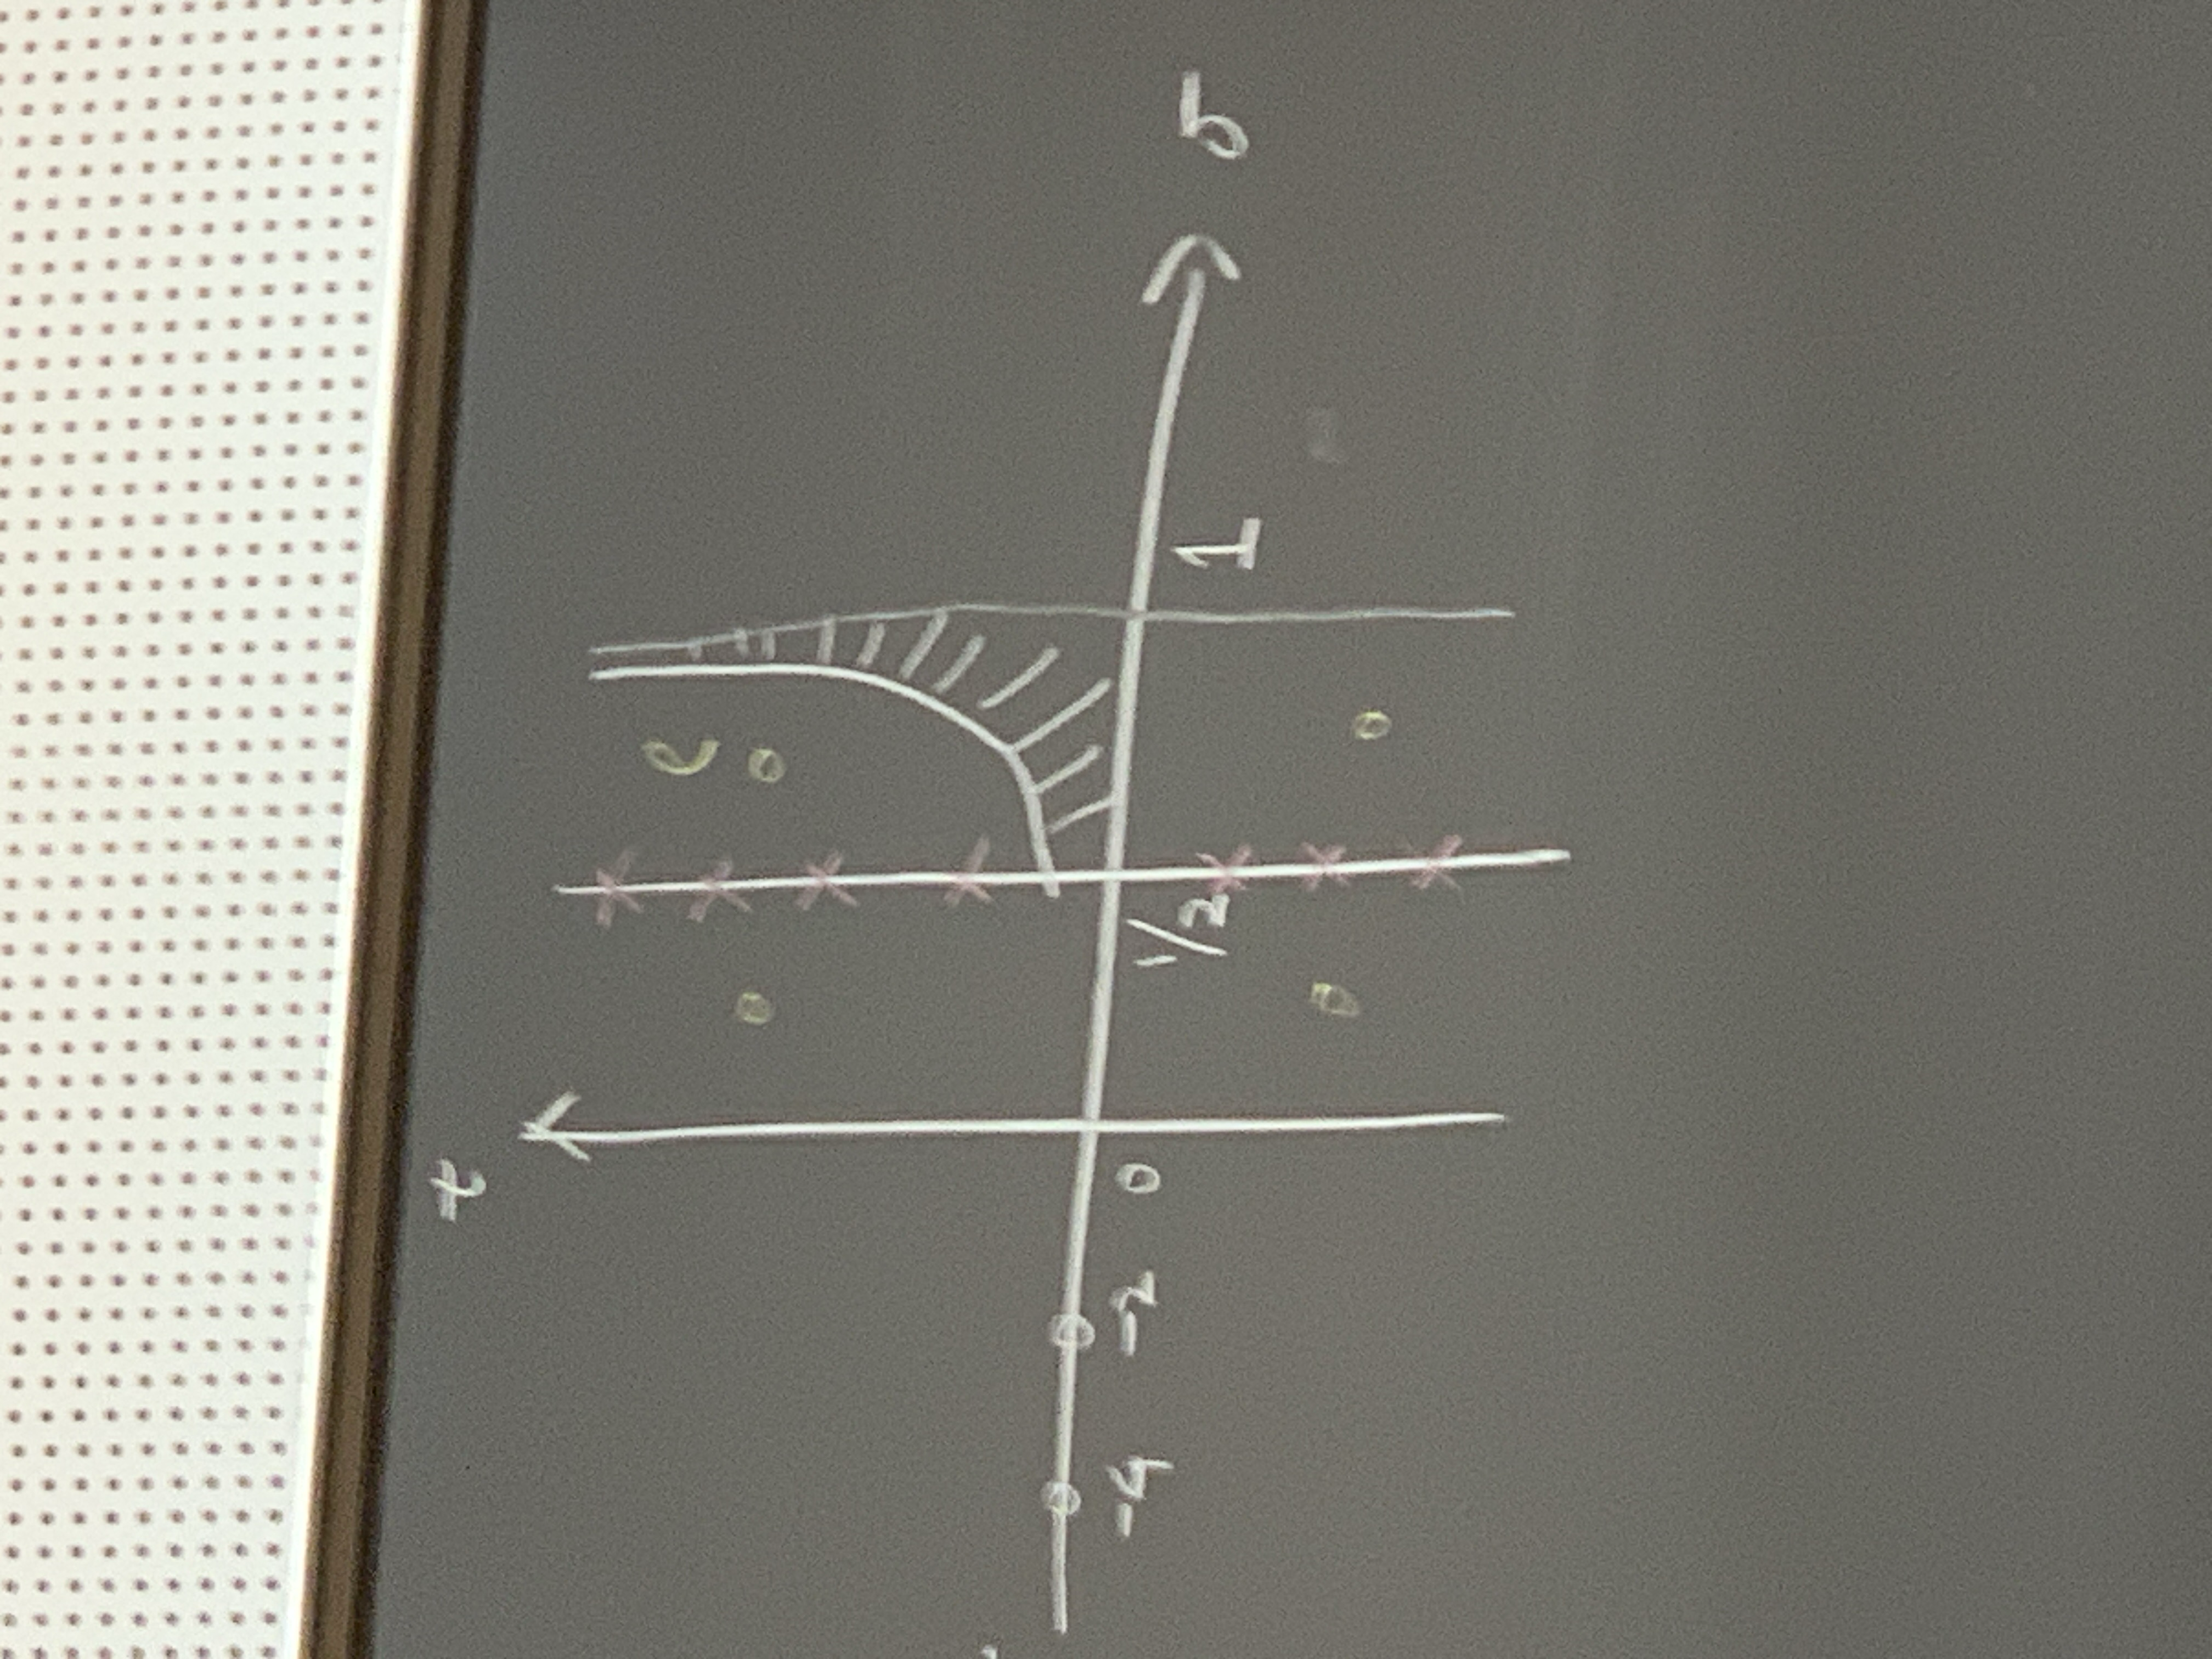
\includegraphics[width=0.5\textwidth]{images/img_20250815_092849}

The basic zero counting function
\begin{equation*}
  N(T) := \# \left\{ \rho = \beta + i \gamma : \zeta(\rho) = 0, \, 0 \leq \beta \leq 1, \, \lvert \gamma \rvert \leq T \right\}
\end{equation*}
satisfies the asymptotic
\begin{equation*}
  N(T) \sim \frac{T}{\pi} \log \frac{T}{2 \pi e}
  \sim \Delta_{[\frac{1}{2} - i T, \frac{1}{2} + i T]} \operatorname{avg} H(s).
\end{equation*}
Hardy (1915) showed that
\begin{equation*}
  N_0(T) := \# \left\{ \rho \text{ as above} : \beta = 1/2 \right\}
  \rightarrow \infty.
\end{equation*}
What methods did Hardy employ to detect zeros on $\sigma = 1/2$?
\begin{itemize}
\item \emph{Sign changes}.  Hardy defined the function $Z(t) := e^{i \theta(t)} \zeta(1/2 + i t)$, which is real-valued for $t \in \mathbb{R}$.  He studied the mean value $\int_I Z(t) \, d t$ of it over some small-ish interval $I$.  The problem with this is that the function fluctuates wildly, so occasional large values swamp the typical behavior.  This is reflected in the fact that Hardy doesn't show a good rate at which $N_0(T)$ tends to infinity.  Later, Hardy--Littlewood refined this approach and showed $N_0(T) \gg T$.
\item \emph{Argument changes}.  Levinson (1974) showed that $N_0(T) > \frac{1}{3} N(T)$ using a different approach.  He started with an Ansatz.  Restrict to the critical line $\sigma = 1/2$.  Suppose, by the functional equation, that we can write the Riemann $\xi$ function as
  \begin{equation*}
    \xi(s) = 2 \Re f(s)
  \end{equation*}
  for a certain entire function $f$.  To understand Levinson's strategy, it's good to draw some pictures.
  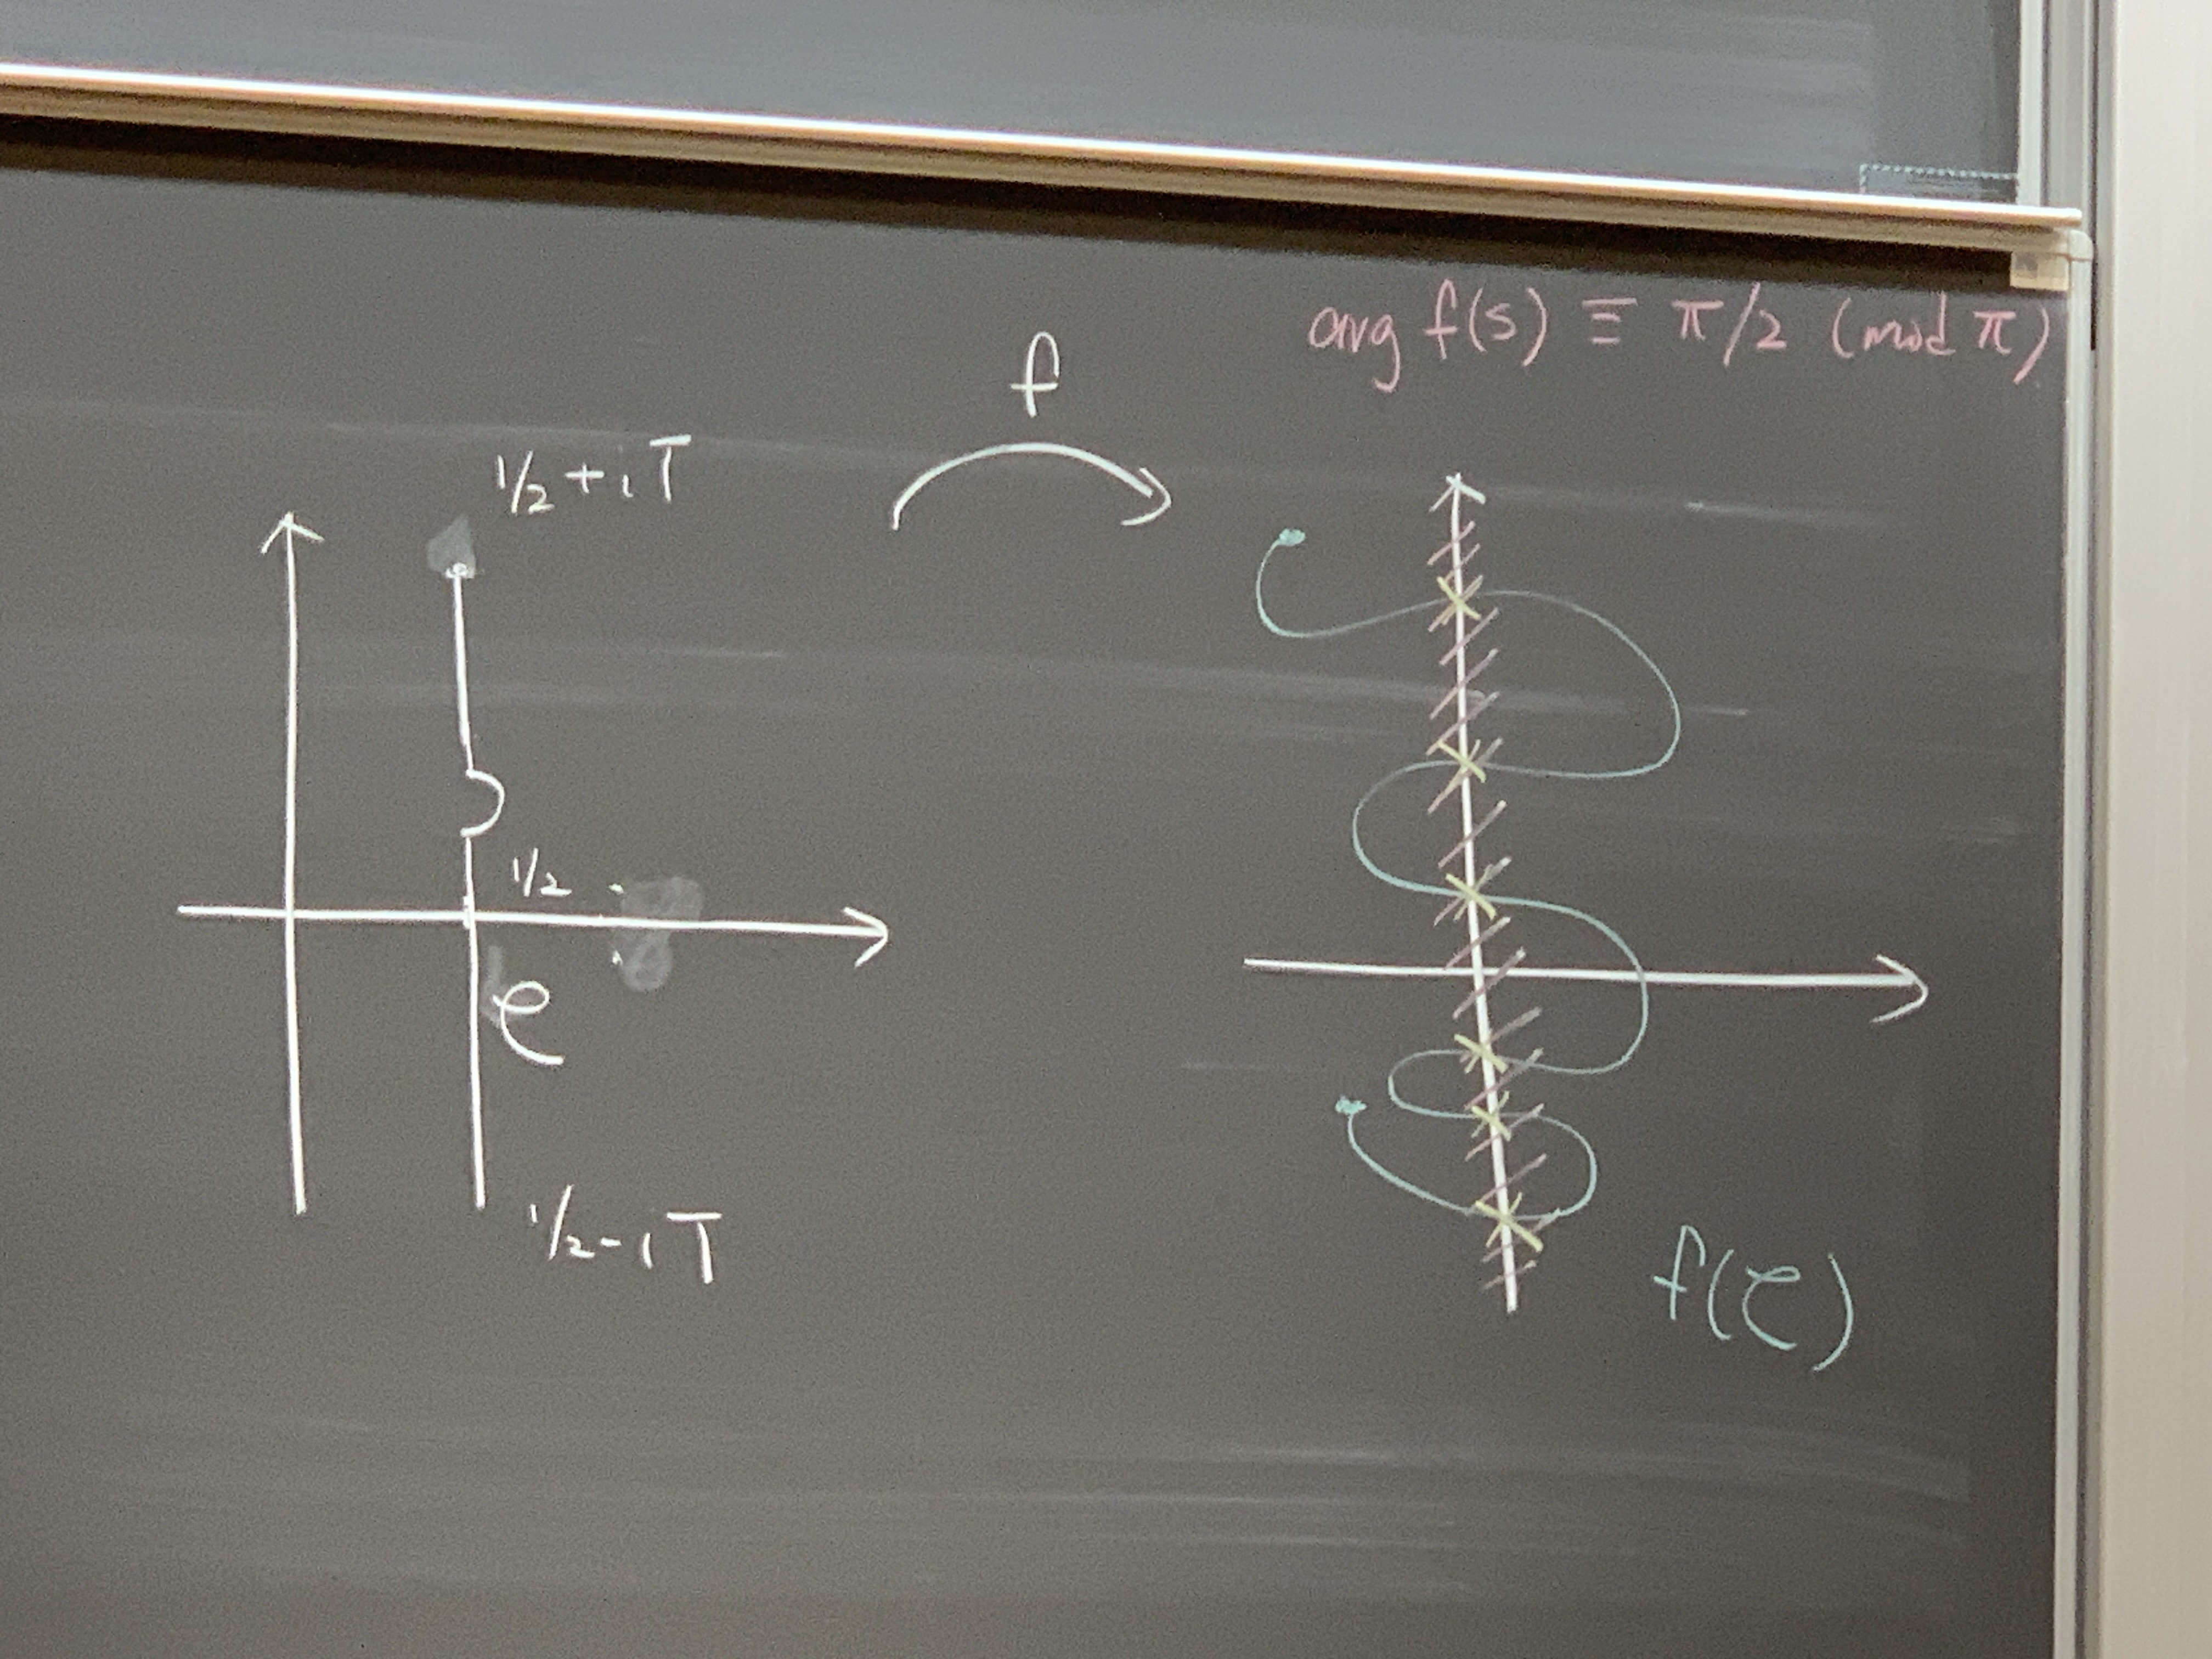
\includegraphics[width=0.5\textwidth]{images/img_20250815_093058}
What Levinson was trying to detect is, when is the argument of $f(s)$ congruent to $\pi /2$ modulo $\pi$, along the indented segment shown in the picture?  The game is detecting when this image curve (depicted in blue) intersect the imaginary axis; that will give zeros on the $1/2$-line.  A naive lower bound for zeros on the critical line is that
\begin{equation}\label{eq:cq6w5cvj0y}
  N_0(T) \geq \frac{1}{\pi} \Delta_{\mathcal{C}} \arg f(s),
\end{equation}
with $\mathcal{C}$ as in the picture.  If you rewrite $f = H G$, with an archimedean (resp.\ non-archimedean) part $H$ (resp.\ $G$), then you can bound the changing argument in \eqref{eq:cq6w5cvj0y} from below by
\begin{equation*}
  \frac{1}{\pi} \Delta_{\mathcal{C}} \arg H(s) + \frac{1}{\pi} \Delta_{\partial R} \arg G(s),
\end{equation*}
using the boundary of the rectangle $R$ indicated below.
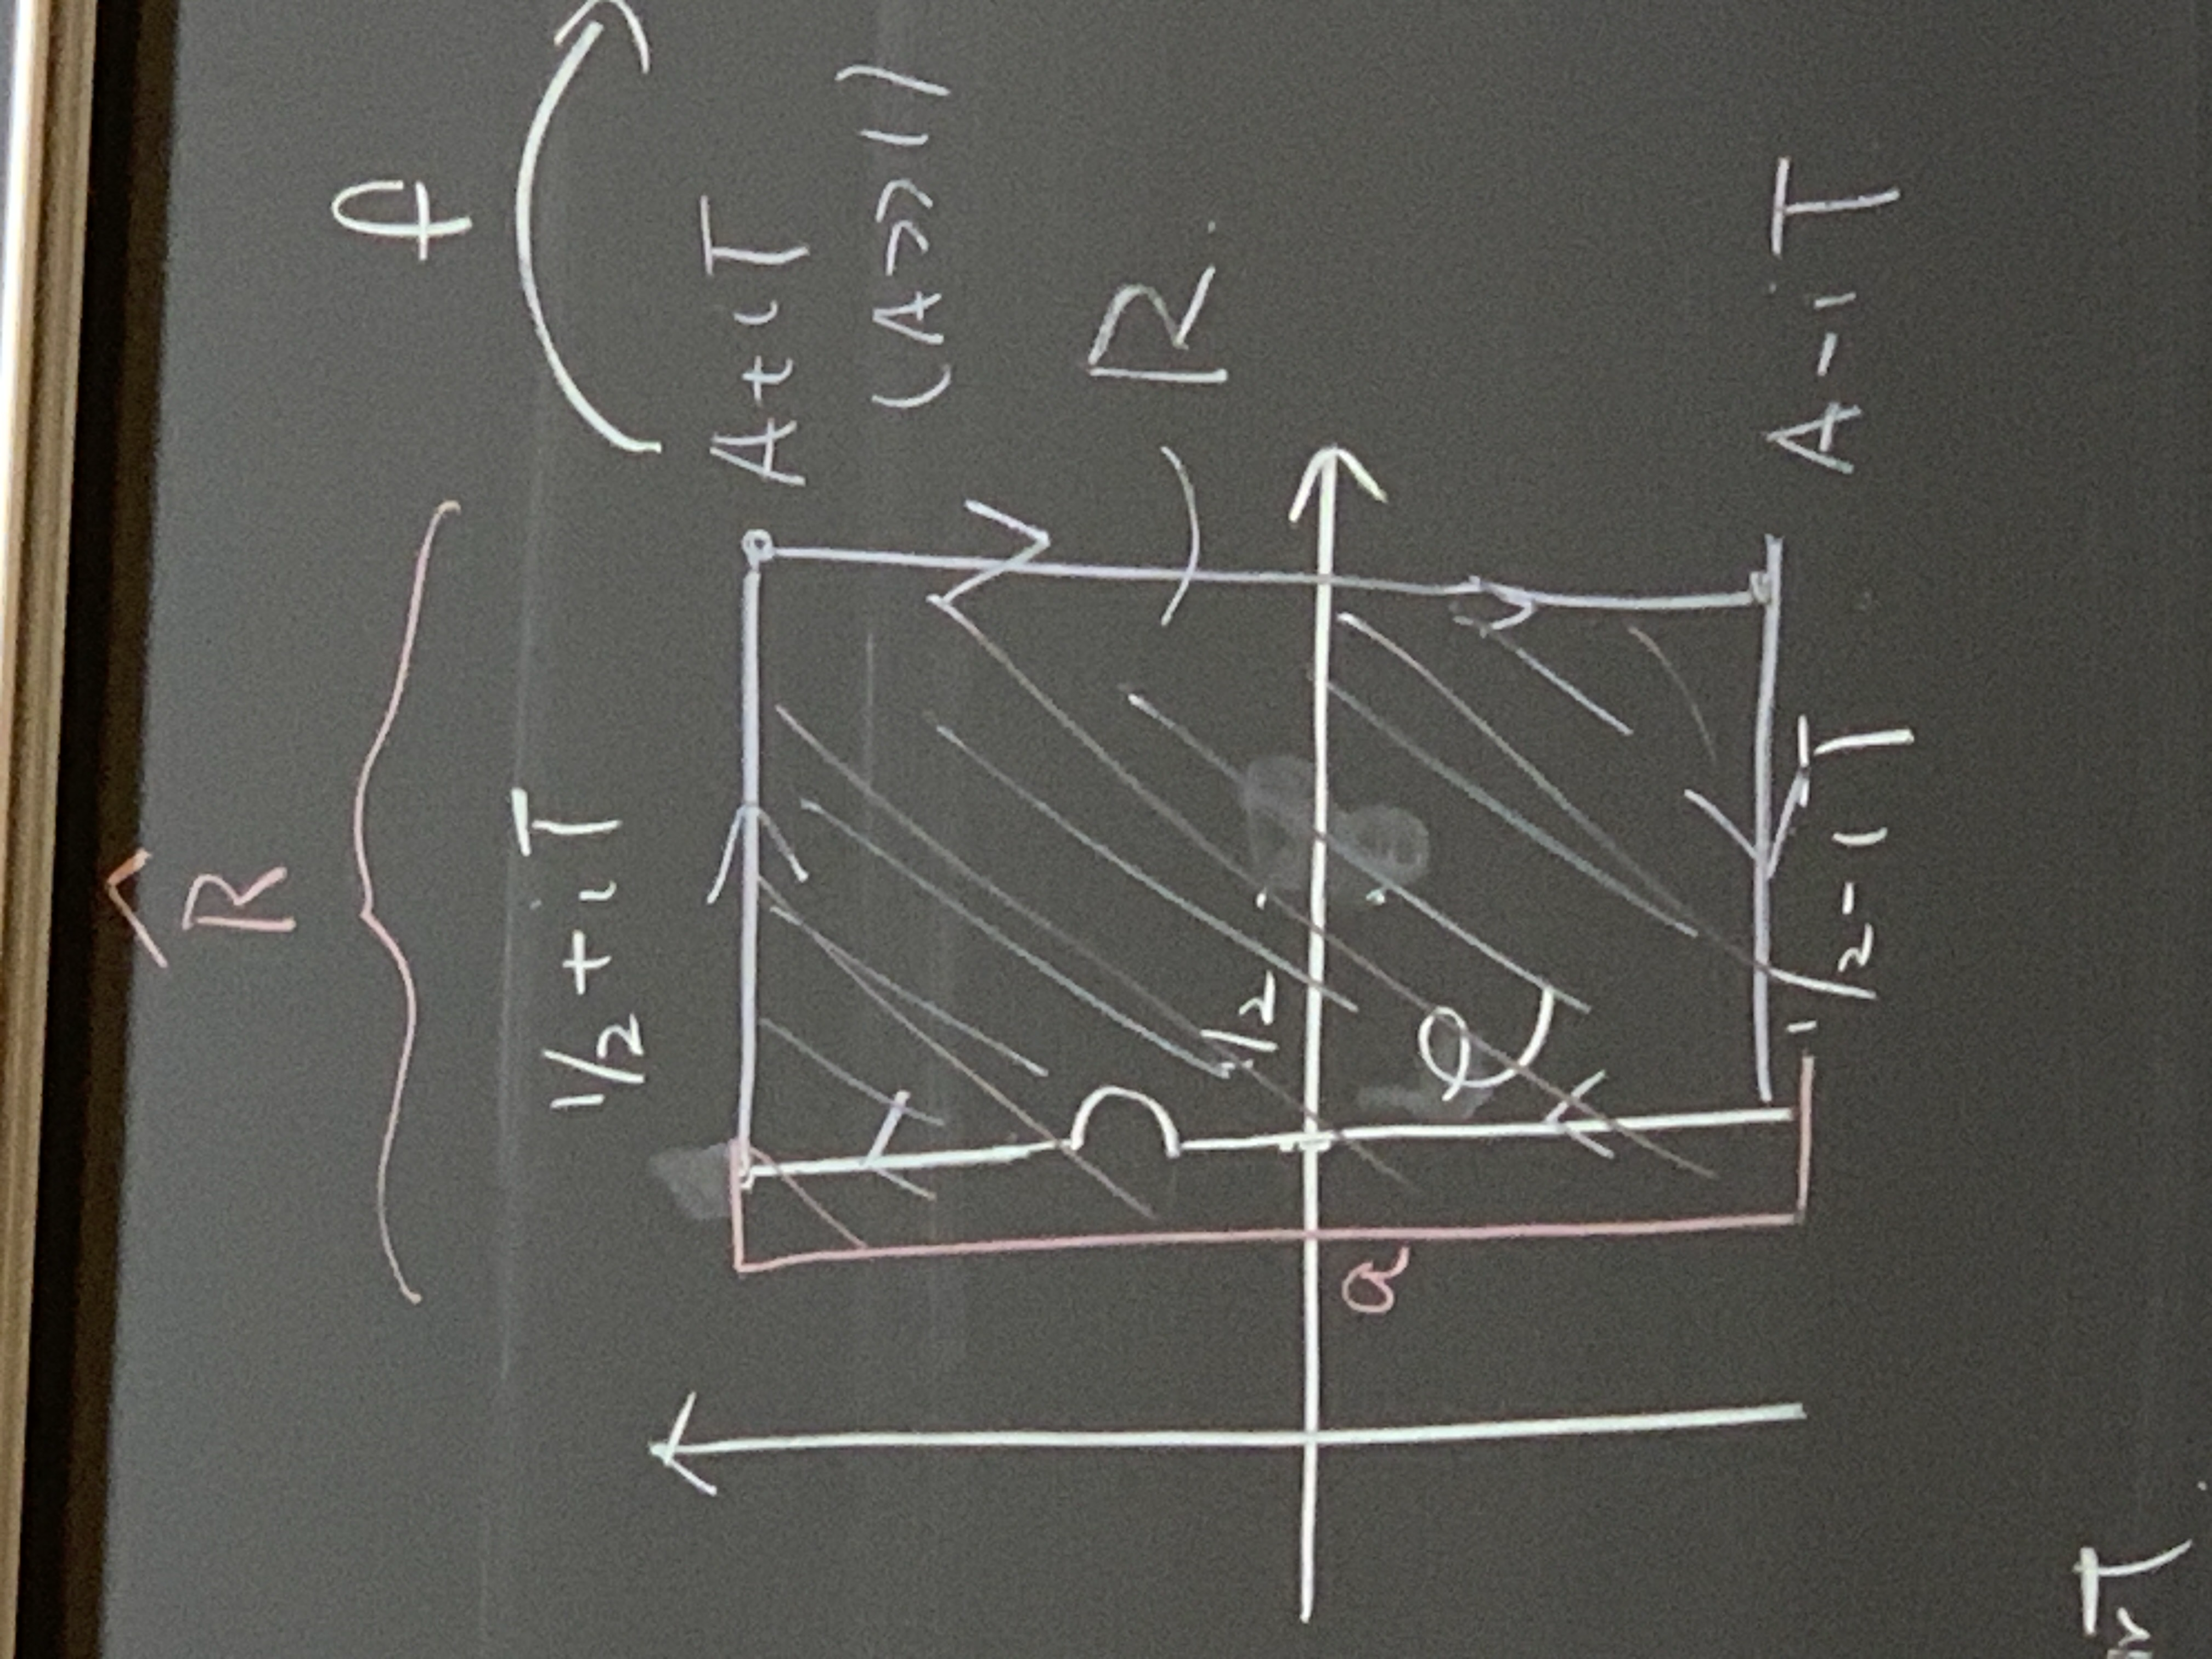
\includegraphics[width=0.5\textwidth]{images/img_20250815_093455}

One can then further bound the above below by $N(T) - 2 N_R(G)$ up to some small error.  But, \emph{a priori}, for this strategy, there's no guarantee that this quantity is positive.  That's the gamble for Levinson.  But at least this strategy says how to approach a problem via the mean value of the Riemann $\xi$ function, for example.  To make the translation, we need to use a gift from Denmark, Jensen's inequality.  To count the zeros, we use that, with $a$ as in the above picture,
\begin{equation*}
  (1/2 - a) N_R(G) \leq \frac{1}{2 \pi} \int_{\partial \hat{R}} \log \lvert G(s) \rvert \, d s
  =
  \frac{1}{2 \pi} \frac{1}{2} \int_{\partial \hat{R}} \log \lvert G(s) \rvert^2 \, d s.
\end{equation*}
One then uses something by Littlewood, roughly a mean value theorem for $G$.  We don't know how to compute the moment, but we can use log-convexity to pull the log outside the moment, leading to
\begin{equation*}
  \leq \frac{1}{4 \pi} \log \int_{a - i T}^{a + i T} \lvert G(s) \rvert^2 \, d t.
\end{equation*}
\end{itemize}

To do better, we need to use another gift from Denmark -- mollifiers, originally used by Bohr.  A mollifier $M$ only introduces more zeros, so
\begin{equation*}
  (\tfrac{1}{2} - a) N_R(G) \leq(\tfrac{1}{2} - a) N_R(G M) \leq \dotsb.
\end{equation*}
You would like to take $M = \zeta^{-1}$, but this isn't practical, so one instead takes something like a truncation.  What Levinson did was to take
\begin{equation*}
  M(s) := \sum_{h \leq y} \frac{M(h)}{h^{s + 1/2 - a}} \frac{\log(Y / h)}{\log Y}
  \approx \zeta(1/2 + i T)^{-1} \quad(Y = T^0).
\end{equation*}
Assuming RH, there is an equivalent formulation due to Speiser in 1935 which says that all the zeros of the derivative of $\zeta '(1 - s)$ are all to the left of the $1$-line.  Later on, Levinson and Montgomery show something even more precise: if you have a zero $\rho '_r$ for $\zeta '$ to the right of the critical line, then you get a zero of $\zeta$ to the left of the critical line, with control over the distances:
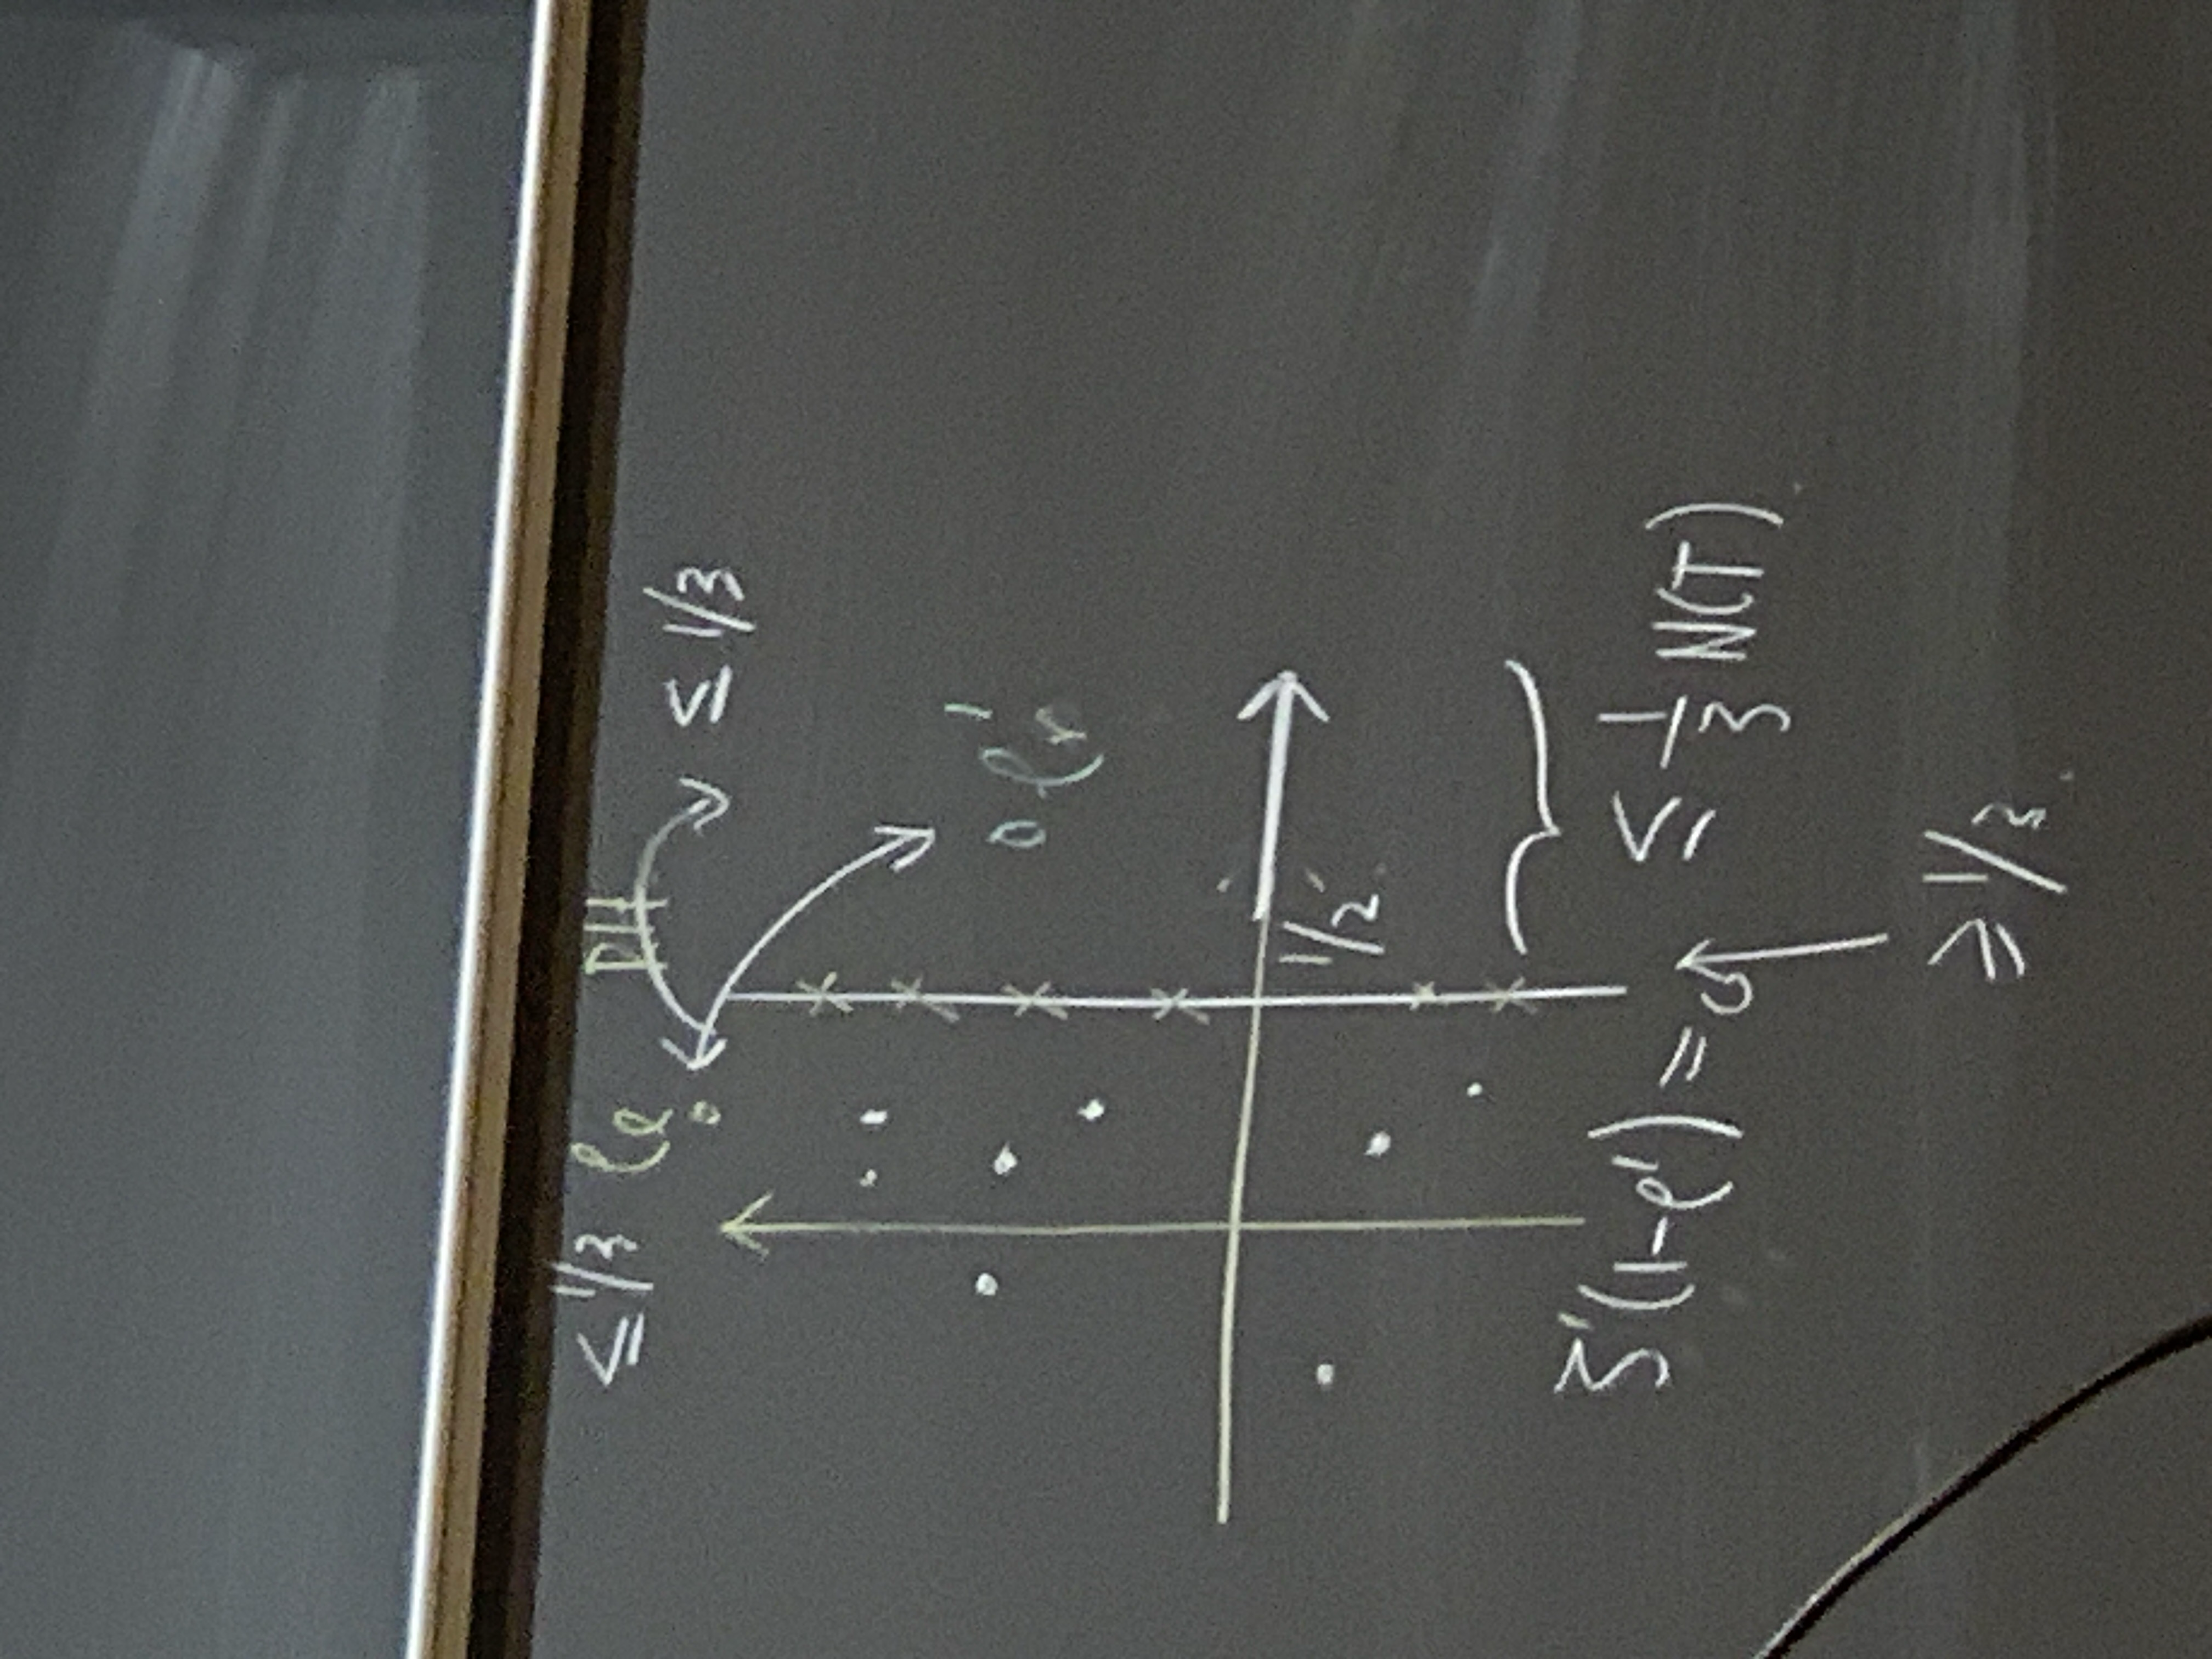
\includegraphics[width=0.5\textwidth]{images/img_20250815_094533}
Levinson then takes $f(s) =(\xi(s) + \lambda \xi '(s)) / 2$ and shows that, for some shifts $\alpha$ and $\beta$,
\begin{equation*}
  \int_0^T \zeta(1/2 + \alpha + i t) \zeta(1/2 + \beta - i t) \Bigl( \frac{k}{h} \Bigr)^{i t}
  \, d t
  = \mathrm{MT}(h k) + \mathcal{E}(h, k)
\end{equation*}
as $T \rightarrow \infty $.  Here $\mathcal{E}$ is understood as an error term in the bilinear sense.

We want to do something like this more generally.  We consider
\begin{equation*}
  \sum_{q \sim Q} \sum_{\chi(q)}^\ast
  \chi(h) \overline{\chi}(k)
  \mathcal{M}_{\alpha, \beta}(h, k; \pi),
\end{equation*}
where $\pi \in \mathcal{A}_0(\PGL (3))$  and
\begin{equation}\label{eq:cq6w5d17ud}
  \mathcal{M}_{\alpha, \beta}(h, k;\pi) := \int_0^T L(1/2 + \alpha + i t, \pi \times \chi)
  L(1/2 + \beta - i t, \bar{\pi} \times \bar{\chi})
  \Bigl( \frac{k}{h} \Bigr)^{i t} \, d t.
\end{equation}
\begin{theorem}[Conrey, Kwan, Lin, Turnage-Butterbaugh]
  Suppose $\pi \in \mathcal{A}_0(\PGL(3) / \mathbb{Q})$ such that either
  \begin{itemize}
  \item $\pi \simeq \tilde{\pi}$, or
  \item $30 \mid q_\pi$ and  $\sum_{n \leq x} \frac{\lvert \lambda_\pi(n) \rvert^4}{n} \ll_\pi x^\eps$.
  \end{itemize}
  Suppose $\theta \in [0,1/2)$ and
  \begin{equation}\label{eq:cq6w5d7akn}
    Q^\eps \ll T \ll Q^{\frac{1 - 2 \theta}{3 - 2 \theta} - \eps},
  \end{equation}
  with $Q \rightarrow \infty$.  Let $(\lambda_h)$ be complex numbers such that
  \begin{enumerate}[(a)]
  \item\label{enumerate:cq6w5d4pra} $\lambda_h \ll h^{\gamma_\theta}$ and $\sum_{n \leq(T Q)^\theta} \frac{\lvert \lambda_h \rvert^{2 m}}{h} \ll(T Q)^\eps$ for $m = 1, 2$.
  \end{enumerate}
  Then
  \begin{equation*}
    \mathcal{M}_{\alpha, \beta}(h, k; T) =(\text{expected } \mathrm{MT} \asymp T Q^2)
    + \mathcal{E}_{\alpha, \beta}(h, k),
  \end{equation*}
  where
  \begin{equation*}
    \sum_{h, k \leq(T Q)^\theta}
    \frac{\lambda_h \overline{\lambda_k}}{\sqrt{h k}}
    \mathcal{E}_{\alpha, \beta}(h, k)
    \ll(T Q)^{7/4 + \theta / 2 + \eps}.
  \end{equation*}
\end{theorem}
\begin{theorem}[CKLT-B and Farmer]
  For $\pi$'s as above and $\eps > 0$ sufficiently small, there are $\geq(11.4 - \O(\eps))$ percentage of zeros with $\lvert \gamma \rvert \leq Q^\eps$ for the family $\{L(s, \pi \times \chi) : \chi(q)^\ast, \, q \sim Q\}$ that are on the critical line.
\end{theorem}
We emphasize that our results are unconditional for $\pi = \bar{\pi}$, independent of GRC.  It's also fully unconditional for $\mathrm{GL}(2)$ Maass forms.  We note that there's no hope to asymptotically evaluate \eqref{eq:cq6w5d17ud} when $T$ is too small and $Q$ is large.  This motivates the assumption \eqref{eq:cq6w5d7akn}.
We can't take $T$ too large, because then we would encounter difficult shifted convolution sums.  So the moral of the story is that this result is strong in the $Q$-aspect, while we only get ``something'' in the $T$-aspect (e.g., nothing beyond $Q^{1/3}$).

The idea of the proof is to use approximate functional equation and orthogonality.  This gives
\begin{equation*}
  \mathcal{M}(h, k, \pi) \approx T \sum_{c d \sim Q} \mu(c) \phi(d)
  \sum_{
    \substack{
      m n \ll(T Q)^3  \\
      m h \equiv n k(d) \\
      m h \approx n k
    }
  }
  \frac{\lambda_\pi(m) \lambda_{\tilde{\pi}}(n)}{\sqrt{m n}}.
\end{equation*}
Suppose for instance that $T \sim Q^\eps$ and $0 < 1/2 - \O(\eps)$.  We truncate and re-expand according to whether $c > C$ or not, where $C \approx Q^\eps$.  We get
\begin{equation*}
  \mathcal{M}_{c > C} \approx \sum_{
    \substack{
      c > C  \\
      d \ll Q / C      
    }
  }^\ast \mu(c) \sum_{\psi(d)}^\ast \psi(h) \overline{\psi}(k)
  \int_{t \approx T}
  \sum_{m n \ll(T Q / C)^{3/2}}
  \frac{\lambda_\pi(m) \lambda_{\tilde{\pi}}(n)}{\sqrt{m n}}.  
\end{equation*}
We then switch and re-expand and use arithmetic: writing $m h = n k + d l$, we see that for $m h \neq n k$, we have $\ell \ll \frac{m h - n k}{d} \ll \frac{c}{Q}(T Q)^{3/2 + \theta}$.  So the whole point of this hyperbola trick is that the length is now much shorter, by a factor of $Q$.  This enables divisor switching.  Because we're doing the aspect where $Q \rightarrow \infty$, we can drop the condition $m h \neq n k$.  After dropping this condition, we can reexpand (mod $\ell$) as above.  This leads to a problem in multiplicative number theory.  The game is, how do you use the hybrid large sieve for the rest of the sums, making sure that the argument is independent of GRC.  Previous relevant work was done by Conrey--Iwaniec--Sound.  They used the bound $\tau_3(n) \ll n^\eps$ all the time.  For a cuspidal automorphic representation, we only have the much weaker bound $\lambda_\pi(n) \ll n^{5/4 + \eps}$.  So one needs to overcome that crutch.

\bibliography{refs}{} \bibliographystyle{plain}
\end{document}
